%!TEX root = ../dissertation.tex

\chapter{Results and Discussion}
\label{chapter:evaluation}

This chapter presents the experimental evaluation of uncertainty in \gls{MOSA}'s multi-omic reconstructions. Section \ref{sec:data} first describes the datasets and the transformations applied to them. The analysis is then divided into two parts, each corresponding to one of the two uncertainty estimation strategies introduced in Chapter \ref{chapter:Uncertainty_Estimation}, these being Latent Space Sampling with decoding and Monte Carlo Dropout. For each method, the resulting predictive distributions are assessed across the seven omics using sharpness, calibration and scoring-rule metrics and by comparing in-sample and out-of-sample reconstructions.


\section{Data Description and Transformation} \label{sec:data}

This section describes the seven datasets whose reconstructions are analysed in this chapter and the transformations applied to them before the uncertainty quantification metrics were calculated, and defines the in-sample and out-of-sample subsets compared throughout the analysis. These characteristics, such as data type, dimensionality and percentage of missing values, are referred to throughout the analysis of the results.

\subsection{Description of the Datasets} \label{chapter:Data} \label{chapter:Data_Description}


This subsection outlines the origin and characteristics of the seven datasets used in MOSA as well as in this thesis. The datasets here described are primarily derived from the Cancer Dependency Map (DepMap) project. This project is a collaborative initiative between the Broad Institute of MIT and Harvard, and the Wellcome Sanger Institute in the United Kingdom. It aims to systematically profile the genetic landscape and phenotypic vulnerabilities of thousands of cancer cell line models. By centralising clinical, genetic and functional data the consortium provides a robust framework for investigating cancer dependencies and prioritising therapeutic targets. 


The multi-omic integration strategy encompasses seven distinct biological and phenotypic layers, ranging from the fundamental genetic code to functional responses to perturbations. Together, these seven datasets encompass 1,523 cancer cell line models, each spanning at least two omics. Of these 1,523, 25.8 percent of the cell lines are present in all seven datasets.

Transcriptomics data provides information on mRNA gene expression for over 15,000 genes, acting as a primary indicator of cellular activity. This dataset is gathered from both the Sanger and Broad Institutes, utilising RNA-seq measurements that are typically reported as \gls{TPM} and log2-transformed to represent a continuous distribution.

Methylation profiling focuses on DNA methylation, an epigenetic mechanism involving the addition of a methyl group to cytosine. This is essential for understanding gene silencing and regulation. Sourced from the Sanger Institute and measured using the Illumina HumanMethylation450 BeadChip, the data is reported as beta values ranging from zero, hypomethylated, to one, hypermethylated. This layer includes 14,608 genes across 906 cell lines.

Proteomics measures the relative abundance of thousands of proteins across cell lines using mass spectrometry. Specifically, the ProCan-DepMapSanger dataset utilises \gls{DIA} and the DIA-NN tool to provide a relative protein quantitation. This layer is particularly challenging due to high missing values (often exceeding 30 percent) resulting from technical limitations in detecting lowly abundant proteins. The proteomics dataset includes 4,922 genes across 949 cell lines.

Metabolomics characterises the intracellular metabolites that act as substrates, intermediates and products of cellular metabolism. Profiling of 225 polar and lipid species is performed using \gls{LC-MS}. This resource, originally published by the Broad Institute, provides insights into the metabolic diversity of cancer across more than 20 cancer types for 900 cell lines.

Drug Response represents a phenotypic layer measuring the sensitivity of cell lines to various compounds, expressed as the \gls{IC50}, the concentration required to inhibit a biological process by half. The data is collated from the GDSC1 and GDSC2 screens, representing a spectrum of common and rare adult and childhood cancers. This dataset contains information for 810 drugs across 993 cell lines.

CRISPR-Cas9 data captures gene essentiality or "fitness scores" derived from genome-scale knockout screens where a gene is classified as essential if its removal leads to cell death. The datasets from Sanger and Broad are combined and batch-corrected using ComBat to account for differences in library design and assay length. This layer encompasses 17,931 gene fitness scores for 992 cell lines.

Copy number alterations form a crucial component of the genomics layer, measuring \glspl{SCNA} such as gene amplifications and deletions. These alterations are detected by integrating \gls{WES} data through the GATK CNV pipeline and PureCN software. For integration within the MOSA framework, total Copy number values are categorised into five ordinal states: deletion, loss, neutral, gain, or amplification. This dataset encompasses 777 features for 1,198 cell lines.

A summary of the key information of these seven datasets can be seen in Table \ref{tab:datasets_description}.

\begin{table}[h!]
\centering
\small
\begin{tabular}{|>{\centering\arraybackslash}m{2.2cm}|>{\centering\arraybackslash}m{2.9cm}|>{\centering\arraybackslash}m{1.6cm}|>{\centering\arraybackslash}m{2.1cm}|>{\centering\arraybackslash}m{1.8cm}|>{\centering\arraybackslash}m{1.8cm}|}
\hline
\textbf{Omic} & \textbf{Data Description} & \textbf{Features \& Samples} & \textbf{Percentage of Missing Values} & \textbf{Data Type} & \textbf{Data Source} \\ \hline
Transcriptomics & mRNA gene expression levels & 15,278 $\times$ 1,240 & 0\% & Continuous & Sanger \& Broad \cite{GarciaAlonso2018} \\ \hline
Methylation & DNA methylation beta values & 14,608 $\times$ 906 & 0\% & Continuous & Sanger \cite{Iorio2016} \\ \hline
Proteomics & Relative protein abundance & 4,922 $\times$ 949 & 47.92\% & Continuous & Sanger \cite{Goncalves2022} \\ \hline
Metabolomics & Intracellular metabolite levels & 225 $\times$ 900 & 9.29\% & Continuous & Broad \cite{Li2019} \\ \hline
Drug Response & Compound sensitivity (IC50) & 810 $\times$ 993 & 25.81\% & Continuous & Sanger \cite{Yang2013,Iorio2016} \\ \hline
CRISPR-Cas9 & Gene essentiality fitness scores & 17,931 $\times$ 992 & 0.94\% & Continuous & Sanger \& Broad \cite{Behan2019} \\ \hline
Copy number & Somatic copy number alterations & 777 $\times$ 1,198 & 2.55\% & Categorical & Sanger \& Broad \cite{Iorio2016} \\ \hline
\end{tabular}
\caption{Table outlining the seven datasets' key characteristics.}
\label{tab:datasets_description}
\end{table}

\subsection{Data Transformation} \label{chapter:Data_transformation}

Due to the different natures of the datasets used, transformations to the data were required before the uncertainty quantification metrics could be calculated. These transformations were applied to both enable and simplify the analysis of each individual omic, while also allowing for these results to be compared consistently across omics. 

For each of the omics described in Section \ref{chapter:Data}, other than the raw data, there are three additional datasets that also underwent these transformations. Firstly, there is a deterministic model reconstruction of the data which corresponds to the model's reconstruction output. These output datasets have the same number of features as the corresponding raw datasets while having all the cell lines reconstructed, thus having 1,523 observations each. Additionally, there are two three-dimensional datasets, one for each of the sampling methods described in Sections \ref{Latent_Space_Sampling} and \ref{Monte_Carlo_Dropout}. These datasets have the same feature and observation dimensions as their deterministic reconstruction counterparts, with the 100 sampled reconstructions stored along the third axis. 

The first transformation applied to the data was the standardisation of cell line model identifiers. Depending on the dataset's origin, cell lines can be identified using either a Sanger identifier, formatted as SIDM-\textit{5 digits}, or a Broad identifier, formatted as ACH-\textit{6 digits}. In some cases, data originating from the Broad Institute can also use a Sanger identifier. To ensure that observations could be matched consistently across all datasets, all cell line identifiers were standardised using the Sanger ID format. Standardising all observations to a single identifier format allows the raw observations, deterministic reconstructions and sampled reconstruction outputs to be aligned and compared correctly across omics.

Another transformation applied to the data was a scaling of the original CRISPR-Cas9 dataset so that it better matched the scale of the deterministic and sampled reconstructions. This scaling was applied to the CRISPR-Cas9 data before it was used as input to the \gls{MOSA} model with the aim of improving the quality of the reconstructed CRISPR-Cas9 values. The transformation used reference behaviour from essential and non-essential genes. For each sample $i$, the median value across essential genes was denoted by $m^{(e)}_i$, and the median value across non-essential genes was denoted by $m^{(n)}_i$. Each original value $x_{ij}$, corresponding to sample $i$ and gene $j$, was then rescaled as seen below.

\begin{equation}
   x'_{ij} = \frac{x_{ij} - m^{(n)}_i}{m^{(n)}_i - m^{(e)}_i}.
\end{equation}

This centres each sample of the CRISPR-Cas9 data so that the median non-essential gene has a value of 0 and the median essential gene a value of $-1$. Applying this transformation to the original dataset ensures all CRISPR-Cas9 datasets used share a common scale.

To allow for simpler analysis and to allow for better comparison between omics, Z-score standardisation was then applied to all continuous datasets. For a value $x_{ij}$ from sample $i$ and feature $j$, the standardised value was calculated as

\begin{equation}
   x_{ij}^{std} = \frac{x_{ij} - \mu_j}{\sigma_j},
\end{equation}

where $\mu_j$ and $\sigma_j$ are the mean and standard deviation of feature $j$ in the corresponding original dataset. The same transformation was also applied to the deterministic reconstruction and sampled reconstruction datasets, using the mean and standard deviation calculated from the original data rather than recalculating these statistics separately for each reconstruction. This was done to preserve a common reference scale between the observed data and the reconstructed datasets.

\subsection{In-Sample and Out-of-Sample Data} \label{sec:in_out_sample}

In this thesis, the train-test split differs from the conventional split used in simpler single-modality models, where whole samples are held out and the model never sees any of their data. Since MOSA is intended to reconstruct omics that are missing for a cell line, only the values of one omic were withheld for a subset of cell lines, while these cell lines remained in the training data with all their other omics and conditional variables. For each of the seven omics, 10\% of the cell lines with measurements of that omic were selected at random and their values for that omic were withheld before training. For these out-of-sample observations, the model reconstructed the withheld values using the information from the remaining available omics. The in-sample observations are the reconstructions of the model trained on all available data, for every cell line with measurements of the target omic. For these observations, the model had access to the target omic during training and reconstruction, so the in-sample results show how closely the model reproduces the data it was trained on. The terms in-sample and out-of-sample used in this chapter thus distinguish reconstructions with and without access to the corresponding omic's values. As the withheld cell lines were selected at random from the same data, the out-of-sample reconstructions should not be interpreted as out-of-distribution. For Proteomics, the Latent Space Sampling and Monte Carlo Dropout out-of-sample results come from two different training runs, with different held-out cell lines (95 and 94, respectively).

\section{Latent Space Sampling with Decoding} \label{LSS_Analysis}

Using the methods described in Chapter \ref{chapter:Uncertainty_Estimation}, MOSA's joint latent space was sampled and decoded, resulting in one hundred samples of the model's data reconstructions across the seven omics studied. This method estimates the aleatoric uncertainty encoded by the VAE in its latent representation and decoded reconstructions as it quantifies the variability encoded from the original data. To assess this uncertainty, three types of uncertainty quantification metrics were computed for the seven reconstructed datasets. Sharpness was measured using PIW for the continuous omics and entropy for the categorical Copy number dataset. Calibration was measured using ENCE for the continuous omics and ECE for Copy number. CRPS and Log Score were used as proper scoring rules for the continuous omics and Copy number respectively.

Both sharpness and scoring were computed along one hundred samples, resulting in a sharpness and scoring value for each data point in each dataset. These datasets thus have the same dimensions as the original raw data. Due to the large dimensionality of this data the analysis of these metrics focuses on feature-wise and observation-wise aggregate values. The mean of each feature's values and the mean of each observation's values were thus computed for both the sharpness and scoring rules, as exemplified in Equation \ref{eq:mean_x_metric}.

\begin{equation} \label{eq:mean_x_metric}
\overline{M}_x
= \frac{1}{|\mathcal{Y}|} \sum_{y \in \mathcal{Y}} M(x,y),
\qquad
M \in \{\mathrm{PIW}, \widetilde{H}, \mathrm{CRPS}, \mathrm{LogScore}\}.
\end{equation}

ENCE and ECE do not require the same type of aggregation, since they are inherently computed at the feature level and already yield a single calibration score for each feature. In contrast, PIW, entropy, CRPS and Log Score first produce a value for each individual data point and therefore require further aggregation along the feature or observation axes. For both the in-sample and out-of-sample analyses, ENCE and ECE were computed using 10 bins. This choice is especially important because the out-of-sample subset contains only 10\% of the observations in each dataset. Using too many bins would therefore increase the risk of sparsely populated bins and unstable calibration estimates, particularly for the out-of-sample data. By fixing the number of bins at 10 for both subsets, the analysis remains more stable and the resulting calibration scores are more directly comparable across datasets and sampling settings.

To provide an initial overview of the uncertainty patterns in each dataset and to facilitate comparison across omics, an additional level of aggregation was computed. Using the previously described feature-wise values, the mean and standard deviation of each metric were calculated for each dataset. This summarised view makes it easier to identify broad differences between in-sample and out-of-sample reconstruction, highlight which omics tend to exhibit higher uncertainty or poorer calibration and establish the main trends before moving to a more granular analysis. It therefore serves as a useful starting point for the later dataset-specific discussion, where the aggregate patterns can be examined in more detail at the feature and observation levels. Throughout this chapter, correlations with an absolute value below 0.3 are described as weak, between 0.3 and 0.7 as moderate, and of 0.7 or above as strong.

%Explicar que se vai começar de uma análise geral, comparando os dados In-sample com OOD, e depois ver uma análise mais focada para cada ómica com highlight das questões mais salientes (Relação com o RMSE [calibration], relação com a correlação entre reconstrução e os dados originais, features ou obs 'outliers', etc)

%1. Mencionar que estou a usar metricas agregadas
%
%2. Ver análise geral da tabela das 3 métricas
%
%3. Ver análise ómica a ómica: Analisar com mais detalhe a sharpness, relação com o RMSE e correlação. Tentar relacionar isto com a natureza dos dados: ver a análise do paper original/ da tese do mofa (por exemplo)
%
%4. Análise disto em relação ao tipo de incerteza, mencionar os problemas gerais outra vez e possíveis soluções.
%

%\subsection{Analysis Overview} \label{LSS_analysis_overview}

\subsection{Analysis of Uncertainty at the Dataset Level}\label{LSS_analysis_overview}


This subsection begins with a general comparison of the continuous data at the dataset level. The purpose of this overview is to identify the main differences between in-sample and out-of-sample reconstructions across omics, while also establishing a baseline comparison between the continuous omics before moving to a more detailed analysis of individual datasets, features and observations. 

Table \ref{tab:uncertainty_summary_all_metrics_sideways} summarises each continuous omic's sharpness, calibration and scoring through the mean and standard deviation of the feature-wise values for both in-sample and out-of-sample data. For all continuous omics, the mean PIW values indicate sharp predictions, while the ENCE values indicate strong miscalibration. For any given model the prediction sharpness should align with the model's error: a prediction with high error should have an equally high interval width for potential predictions. Calibration is dependent on this match between sharpness and predictive error. ECE and ENCE are closer to zero the more prediction variance aligns with prediction error. In this case, it can be seen that in-sample mean ENCE values for all continuous omics range between 15.2, for Metabolomics, and 49.2, for CRISPR-Cas9.

%% Explicar o pq do calibration ser tão alto (em parte devido à formula) e o que seria de esperar para calibration.
%% Copy number isn't very mentioned (due to not being necessarily comparable with the remaining omics), devo mencionar isto mais??
%%% Dizer que normalmente espera-se que out-of-sample data tenha pior miscalibration, o que nao é o caso.

Figure \ref{fig:sharpness_continuous} illustrates the low mean PIW of the continuous features. In-sample mean PIW values are uniformly low, ranging from 0.047 for CRISPR-Cas9 to 0.103 for Metabolomics. These values present a disconnect from the RMSE values of these datasets, as CRISPR-Cas9 in-sample has a mean feature-wise RMSE of 0.756, while for Metabolomics this value is 0.527. This figure also highlights the difference in sharpness out-of-sample. For Metabolomics, Drug Response, Methylation, Proteomics and Transcriptomics, the predictive intervals widen by a factor of four to five out-of-sample, with mean PIW ranging from 0.266 for Methylation to 0.430 for Metabolomics. They remain, however, much narrower than the out-of-sample reconstruction errors, as the calibration values below show. CRISPR-Cas9 is the exception, as its mean PIW only increases from 0.047 to 0.061, so its out-of-sample predictions remain almost as sharp as in-sample.

%Mencionar algo sobre o desvio padrão?

This disconnect between sharpness and reconstruction error is reflected in high ENCE values, illustrated in Figure \ref{fig:calibration_continuous}. All continuous omics have mean in-sample ENCE higher than 1. Out-of-sample, the feature-wise mean ENCE is lower for Metabolomics, Drug Response, Methylation, Proteomics and Transcriptomics, and every individual feature of these omics has a lower ENCE out-of-sample than in-sample, while the mean ENCE of CRISPR-Cas9 increases from 49.2 to 54.5. This reflects the trend seen in PIW values. Additionally, in the five omics where ENCE decreased out-of-sample, the standard deviation of these values also decreased. Despite this decrease in ENCE out-of-sample, which reflects a PIW more aligned with prediction error, mean ENCE values remain large, ranging between 6.29 and 8.22 for these five omics. This miscalibration is analysed in more detail in the following subsection.


The scoring rule values should be interpreted more cautiously. On their own, they do not provide a sufficient basis for judging predictive quality, but they become informative when read jointly with sharpness and calibration and when comparing different reconstructions of the same dataset. Despite the increase in PIW for all continuous omics and the decrease in ENCE for five of them out-of-sample, the CRPS of all omics increases out-of-sample, from 0.39--0.57 to 0.54--0.77. While the decrease in sharpness reduced the overconfidence, improving calibration, CRPS penalised both the lack of sharpness and reconstruction miscalibration. 



\begin{figure}[!h]
    \centering
    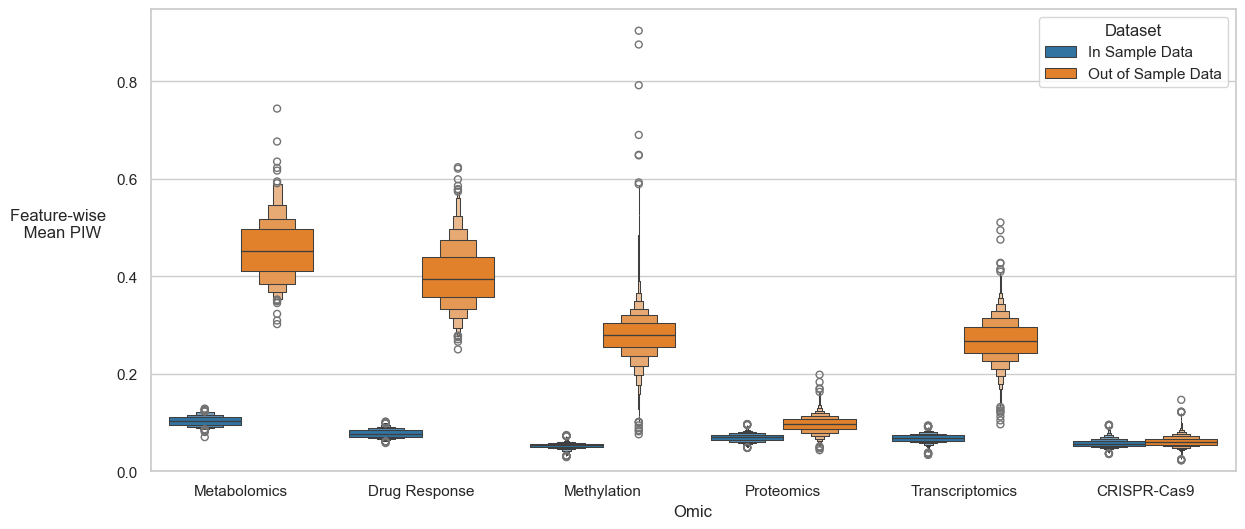
\includegraphics[width=0.9\linewidth]{images/sharpness_continuous.png}
    \caption[Continuous omic sharpness comparison]{Sharpness values across each omic divided between in-sample and out-of-sample data.}
    \label{fig:sharpness_continuous}
\end{figure}

\begin{landscape}
\begin{table}[p]
\centering
\begin{tabular}{|c|cccc|cccc|cccc|}
\hline
\multirow{3}{*}{Dataset} & \multicolumn{4}{c|}{Sharpness}                                              & \multicolumn{4}{c|}{Calibration}                                           & \multicolumn{4}{c|}{Scoring Rules}                                         \\ \cline{2-13}
                         & \multicolumn{2}{c|}{In-Sample}         & \multicolumn{2}{c|}{Out-of-Sample} & \multicolumn{2}{c|}{In-Sample}        & \multicolumn{2}{c|}{Out-of-Sample} & \multicolumn{2}{c|}{In-Sample}         & \multicolumn{2}{c|}{Out-of-Sample} \\ \cline{2-13}
                         & $\mu$  & \multicolumn{1}{c|}{$\sigma$} & $\mu$           & $\sigma$         & $\mu$ & \multicolumn{1}{c|}{$\sigma$} & $\mu$          & $\sigma$          & $\mu$  & \multicolumn{1}{c|}{$\sigma$} & $\mu$          & $\sigma$         \\ \hline
Metabolomics             & 0.103 & \multicolumn{1}{c|}{0.0105}   & 0.430          & 0.0423           & 15.2 & \multicolumn{1}{c|}{4.79}    & 6.29          & 1.10             & 0.391 & \multicolumn{1}{c|}{0.0915}   & 0.636         & 0.0778           \\
Drug Response            & 0.0774 & \multicolumn{1}{c|}{0.0087}   & 0.365          & 0.0425           & 20.8 & \multicolumn{1}{c|}{4.91}    & 6.40          & 1.41             & 0.395 & \multicolumn{1}{c|}{0.0638}   & 0.586         & 0.0847           \\
Methylation              & 0.0529 & \multicolumn{1}{c|}{0.0051}   & 0.266          & 0.0242           & 32.8 & \multicolumn{1}{c|}{10.5}    & 8.22          & 2.03             & 0.414 & \multicolumn{1}{c|}{0.0745}   & 0.543         & 0.0812           \\
Proteomics               & 0.0690 & \multicolumn{1}{c|}{0.0076}   & 0.368          & 0.0399           & 25.2 & \multicolumn{1}{c|}{6.54}    & 6.77          & 2.10             & 0.398 & \multicolumn{1}{c|}{0.0625}   & 0.655         & 0.117           \\
Transcriptomics          & 0.0615 & \multicolumn{1}{c|}{0.0074}   & 0.288          & 0.0317           & 27.9 & \multicolumn{1}{c|}{7.07}    & 7.67          & 1.94             & 0.450 & \multicolumn{1}{c|}{0.0587}   & 0.580         & 0.0922           \\
CRISPR-Cas9              & 0.0467 & \multicolumn{1}{c|}{0.0062}   & 0.0612          & 0.0097           & 49.2 & \multicolumn{1}{c|}{9.77}    & 54.5          & 12.0             & 0.570 & \multicolumn{1}{c|}{0.0415}   & 0.767         & 0.0756           \\ \hline
\end{tabular}
\caption{Summary table of uncertainty metrics by continuous dataset, split by in-sample and out-of-sample subsets.}
\label{tab:uncertainty_summary_all_metrics_sideways}
\end{table}
\end{landscape}

\begin{figure}[!h]
    \centering
    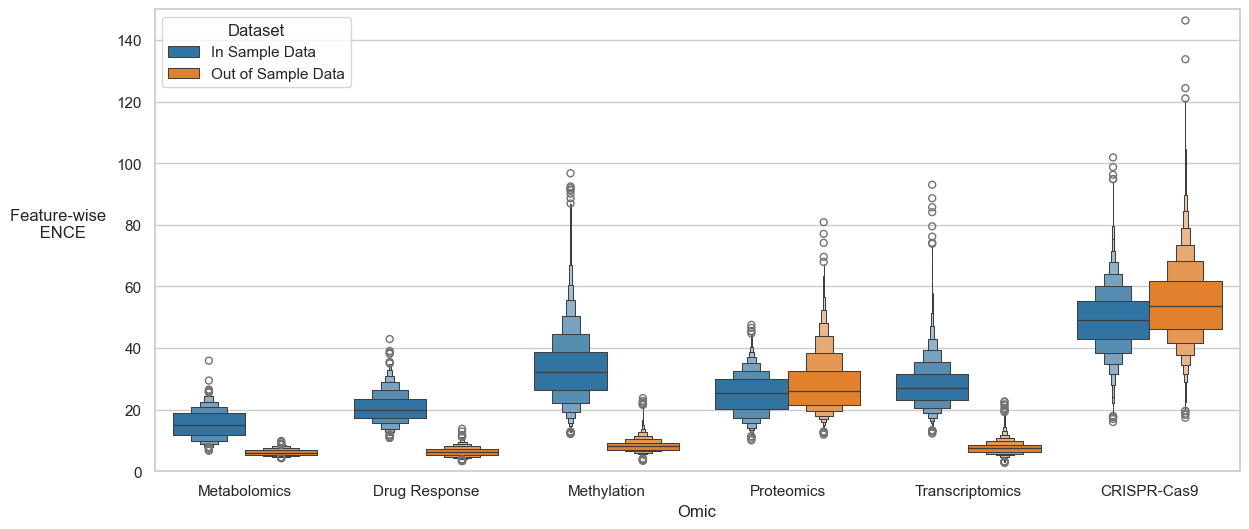
\includegraphics[width=0.9\linewidth]{images/calibration_continuous.png}
    \caption[Continuous omic calibration comparison]{Calibration values across each omic divided between in-sample and out-of-sample data.}
    \label{fig:calibration_continuous}
\end{figure}



% Adicionar: grouped visualization of scoring-rule values together with sharpness or calibration, since scoring rules are not informative on their own.
% Adicionar: schematic summary highlighting omics with the clearest mismatch between sharpness and calibration.


\begin{table}
\centering
\resizebox{\textwidth}{!}{%
\begin{tabular}{|c|cccc|cccc|cccc|}
\hline
\multirow{3}{*}{Dataset} & \multicolumn{4}{c|}{Sharpness}                                              & \multicolumn{4}{c|}{Calibration}                                           & \multicolumn{4}{c|}{Scoring Rules}                                         \\ \cline{2-13}
                         & \multicolumn{2}{c|}{In-Sample}         & \multicolumn{2}{c|}{Out-of-Sample} & \multicolumn{2}{c|}{In-Sample}        & \multicolumn{2}{c|}{Out-of-Sample} & \multicolumn{2}{c|}{In-Sample}         & \multicolumn{2}{c|}{Out-of-Sample} \\ \cline{2-13}
                         & $\mu$  & \multicolumn{1}{c|}{$\sigma$} & $\mu$           & $\sigma$         & $\mu$ & \multicolumn{1}{c|}{$\sigma$} & $\mu$          & $\sigma$          & $\mu$  & \multicolumn{1}{c|}{$\sigma$} & $\mu$          & $\sigma$         \\ \hline
Copy number                & 0.0242     & \multicolumn{1}{c|}{0.0061}       & 0.0343              & 0.0113               & 0.246    & \multicolumn{1}{c|}{0.0652}       & 0.351             & 0.0727                & 7.52     & \multicolumn{1}{c|}{2.15}       & 10.6             & 2.37               \\ \hline
\end{tabular}%
}
\caption{Summary table of uncertainty metrics for Copy number, split by in-sample and out-of-sample subsets.}
\label{tab:uncertainty_summary_copy_number}
\end{table}

\subsection{Analysis of Metabolomics, Proteomics and Copy number}
%Mudar o titulo desta subsection, algo tipo "single omic analysis? Idk"

The omic-wise analysis focuses on three representative omic datasets while integrating comparisons with the remaining omics. Metabolomics is used as the main example of the continuous datasets whose out-of-sample reconstructions become much broader and numerically less miscalibrated, but also harder to reconstruct. Proteomics follows the same pattern, but its high percentage of missing values provides another perspective of analysis. Copy number extends the analysis to categorical data, also focusing on how class imbalance relates to reconstruction uncertainty.

\subsubsection{Analysis of the Metabolomics Dataset}

As shown in Table \ref{tab:uncertainty_summary_all_metrics_sideways}, Metabolomics has the highest mean feature-wise PIW among the continuous omics, and therefore the least sharp predictions, while also having the lowest mean feature-wise ENCE in both settings and the lowest in-sample CRPS. It also shows the largest absolute widening of the predictive intervals between in-sample and out-of-sample reconstructions. Figure \ref{fig:metab_sharp_cal_scor} shows that PIW explains 43\% of the variation in in-sample ENCE, with a weaker relationship out-of-sample ($R^2=0.296$). The tendency for lower ENCE to coincide with lower mean CRPS is expected, as CRPS reflects both sharpness and calibration.

\begin{figure}[!h]
    \centering
    \begin{subfigure}{0.48\linewidth}
        \centering
        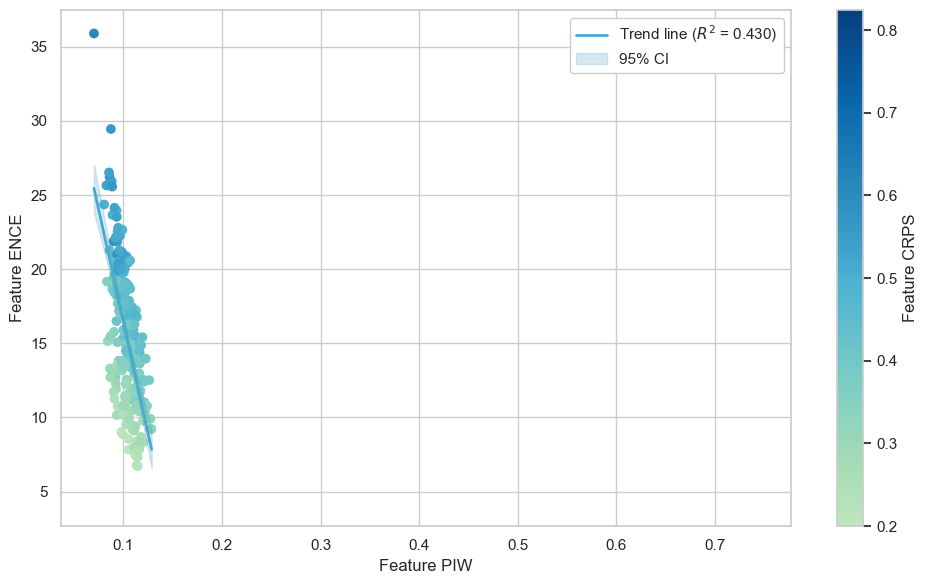
\includegraphics[width=\linewidth]{images/metabolomics_fig/metabolomics_sharp_cal_score_scaled.png}
        \caption{In-Sample data.}
        \label{fig:metab_sharp_cal_scor_in}
    \end{subfigure}
    \hfill
    \begin{subfigure}{0.48\linewidth}
        \centering
        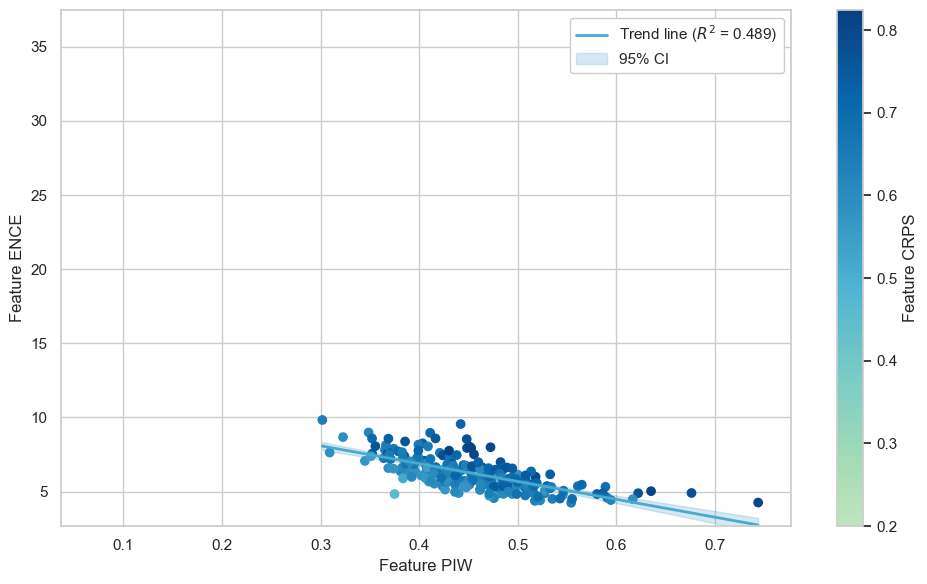
\includegraphics[width=\linewidth]{images/metabolomics_fig/metabolomics_sharp_cal_score_scaled_OOD.png}
        \caption{Out-of-Sample data.}
        \label{fig:metab_sharp_cal_scor_out}
    \end{subfigure}
    \caption[Metabolomics PIW-ENCE scatter plots]{Metabolomics feature-wise scatter plots between PIW and ENCE with CRPS value as a gradient.}
    \label{fig:metab_sharp_cal_scor}
\end{figure}

Figure \ref{fig:corr_metab_metrics} supports this relationship, showing a moderate negative correlation between PIW and ENCE in both reconstructions. In contrast, PIW and CRPS are only moderately correlated in-sample and weakly correlated out-of-sample, while the strong in-sample association between ENCE and CRPS, at 0.89, becomes moderate out-of-sample, at 0.54.

\begin{figure}[!h]
    \centering
    \begin{subfigure}{0.48\linewidth}
        \centering
        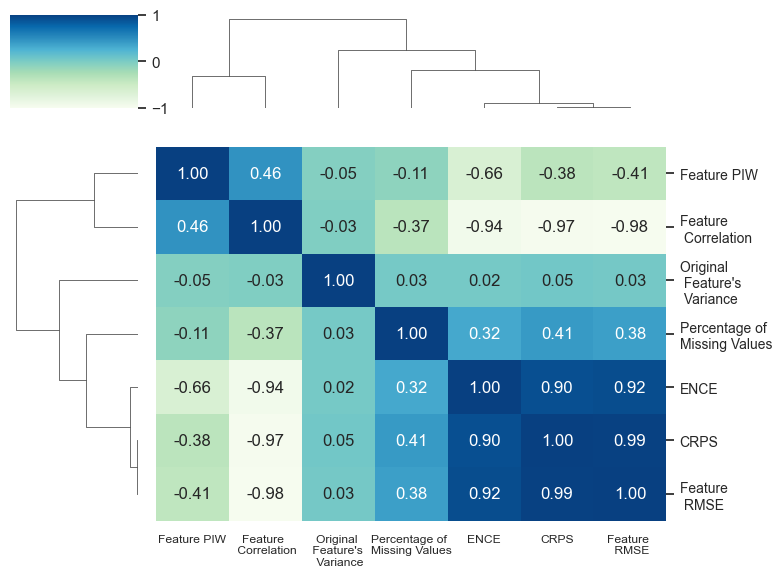
\includegraphics[width=\linewidth]{images/metabolomics_fig/metabolomics_cluster_map.png}
        \caption{In-Sample data.}
        \label{fig:corr_metab_metrics_in}
    \end{subfigure}
    \hfill
    \begin{subfigure}{0.48\linewidth}
        \centering
        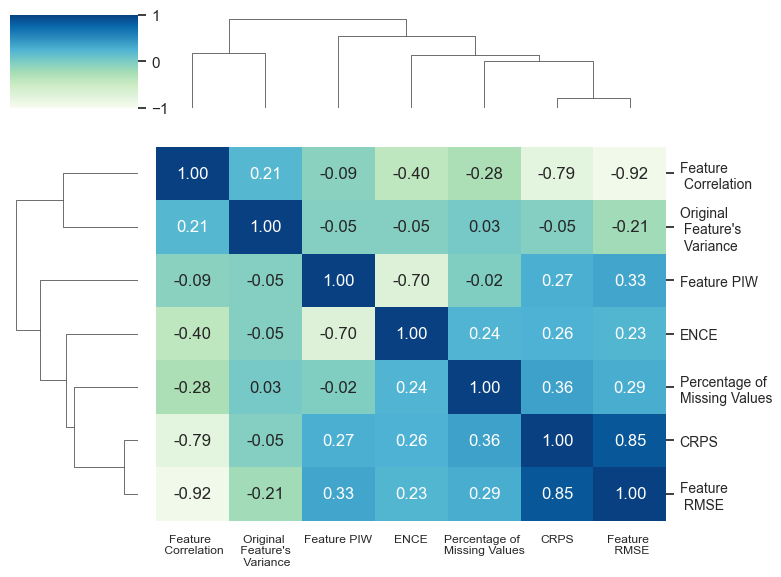
\includegraphics[width=\linewidth]{images/metabolomics_fig/metabolomics_cluster_map_OOD.png}
        \caption{Out-of-Sample data.}
        \label{fig:corr_metab_metrics_out}
    \end{subfigure}
    \caption[Metabolomics uncertainty correlation cluster-map]{Pearson correlation cluster-maps between the feature-wise uncertainty metrics, reconstruction-error metrics, missing-value percentage and original feature variance in Metabolomics.}
    \label{fig:corr_metab_metrics}
\end{figure}


The moderate negative association between mean feature PIW and feature-wise ENCE indicates that the model tends to have wider prediction distributions for better calibrated features. However, the in-sample PIW only ranges between 0.070 and 0.129 compared with 0.319 to 0.552 out-of-sample. Even the widest out-of-sample intervals remain narrow relative to the standardised data, for which a 95\% interval of a standard normal variable has a width of 3.92. Although every feature has a lower ENCE out-of-sample, these values still indicate high miscalibration.

Using the interquartile range as a simple outlier detection method, Adenine was identified as the only in-sample outlier, having the lowest PIW at 0.070 and the highest ENCE at 34.8. Out-of-sample, its ENCE is instead closer to the dataset mean at 7.79, while its PIW is still the lowest of all features, at 0.319.

Predictions with lower PIW accompanied by low ENCE indicate that the model is both accurate and can discern between good and bad predictions. In this case, the in-sample predictions are sharp but have high ENCE, indicating overconfidence, while the out-of-sample PIW is wider but still provides unreliable confidence in feature reconstruction. To better understand this, model error and feature reconstruction were analysed using the \gls{RMSE} and Pearson's correlation between the original features and their respective reconstructions.

%Although very similar measures, as a feature's reconstruction with low RMSE tends to have a high correlation with its ground truth, RMSE and correlation hold different information in the context of biological data. RMSE
%Ia explicar que rmse é só o erro mas que corr mostra mais se a estrutura dos dados é mantida pela reconstrução, e que isso é mais importante (creio)

Figures \ref{fig:metab_cal_rmse_corr_in} and \ref{fig:metab_cal_rmse_corr_out} compare ENCE with feature reconstruction. In-sample, ENCE has a strong relationship with RMSE ($R^2=0.840$), consistent with their correlation of 0.92 in Figure \ref{fig:corr_metab_metrics}. Features with better calibration also tend to have lower reconstruction error. The relationship is weaker out-of-sample ($R^2=0.324$), where it is accompanied by higher RMSE values and lower feature-wise Pearson correlation. The association between better calibration and better reconstruction is therefore strongest in-sample, but it persists out-of-sample.

\begin{figure}[h]
    \centering
    \begin{subfigure}{0.48\linewidth}
        \centering
        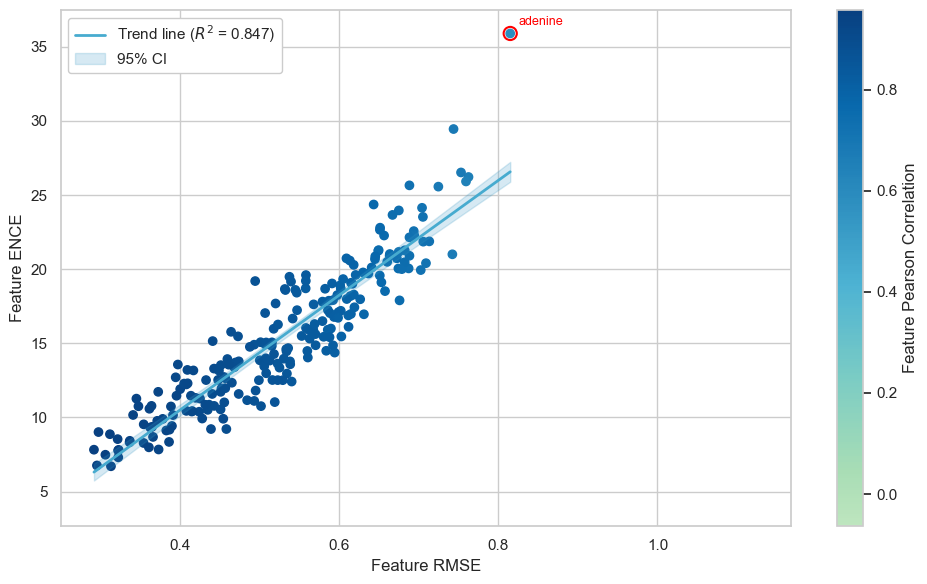
\includegraphics[width=\linewidth]{images/metabolomics_fig/metabolomics_scor_rmse_corr_adenine_scaled.png}
        \caption{In-Sample data.}
        \label{fig:metab_cal_rmse_corr_in}
    \end{subfigure}
    \hfill
    \begin{subfigure}{0.48\linewidth}
        \centering
        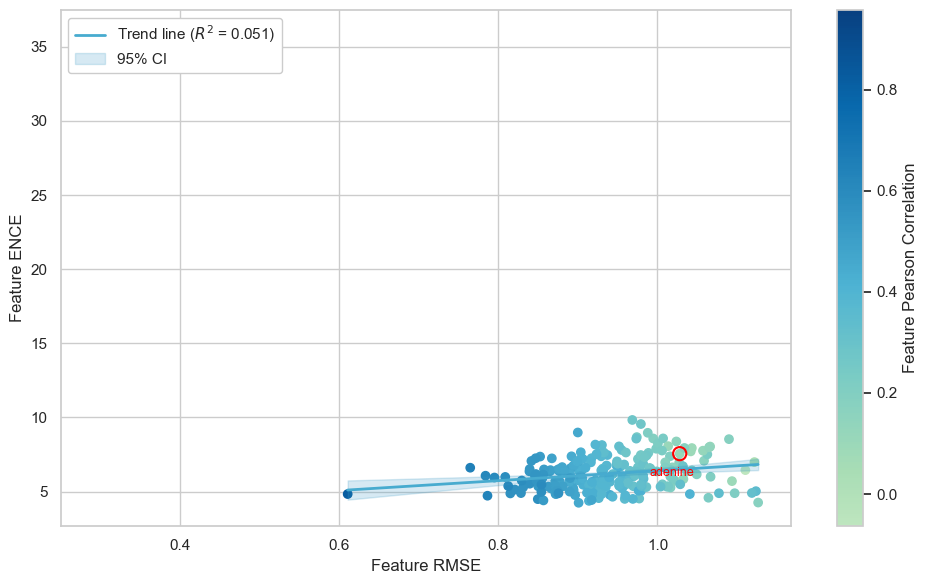
\includegraphics[width=\linewidth]{images/metabolomics_fig/metabolomics_scor_rmse_corr_adenine_OOD_scaled.png}
        \caption{Out-of-Sample data.}
        \label{fig:metab_cal_rmse_corr_out}
    \end{subfigure}
    \caption[Metabolomics RMSE-ENCE scatter plots]{Metabolomics feature-wise scatter plots between RMSE and ENCE with feature correlation as a gradient with equal axes lengths and colouring gradient scales.}
    \label{fig:metab_cal_rmse_corr}
\end{figure}

This behaviour is also representative of Drug Response, Methylation and Transcriptomics, as well as of Proteomics, analysed below. Drug Response shows a similar shift from narrow in-sample PIW values to broader out-of-sample intervals, together with lower out-of-sample ENCE but higher RMSE. Methylation follows the same pattern at a much larger feature scale, reinforcing that the lower out-of-sample ENCE should not be interpreted as better uncertainty estimation on its own. For these omics, broader predictive intervals are more aligned with larger reconstruction errors, while CRPS still indicates worse out-of-sample predictive performance.

To better understand what the ENCE values represent, Figure \ref{fig:metabolomics_calibration_curves} shows the calibration curves of the features with the smallest and largest calibration errors. ENCE bins each feature's data points based on the standard deviation of their predictive distributions and compares the mean RMSE and RMV within each bin. For a perfectly calibrated feature, these values would be equal. While there is a large difference in calibration error between the two groups in Figure \ref{fig:metabolomics_calibration_curves}, all displayed features show overconfident predictions as can be seen by the mismatch in RMSE and RMV mean bin values.


\begin{figure}[!ht]
    \centering
    \begin{subfigure}{0.48\linewidth}
        \centering
        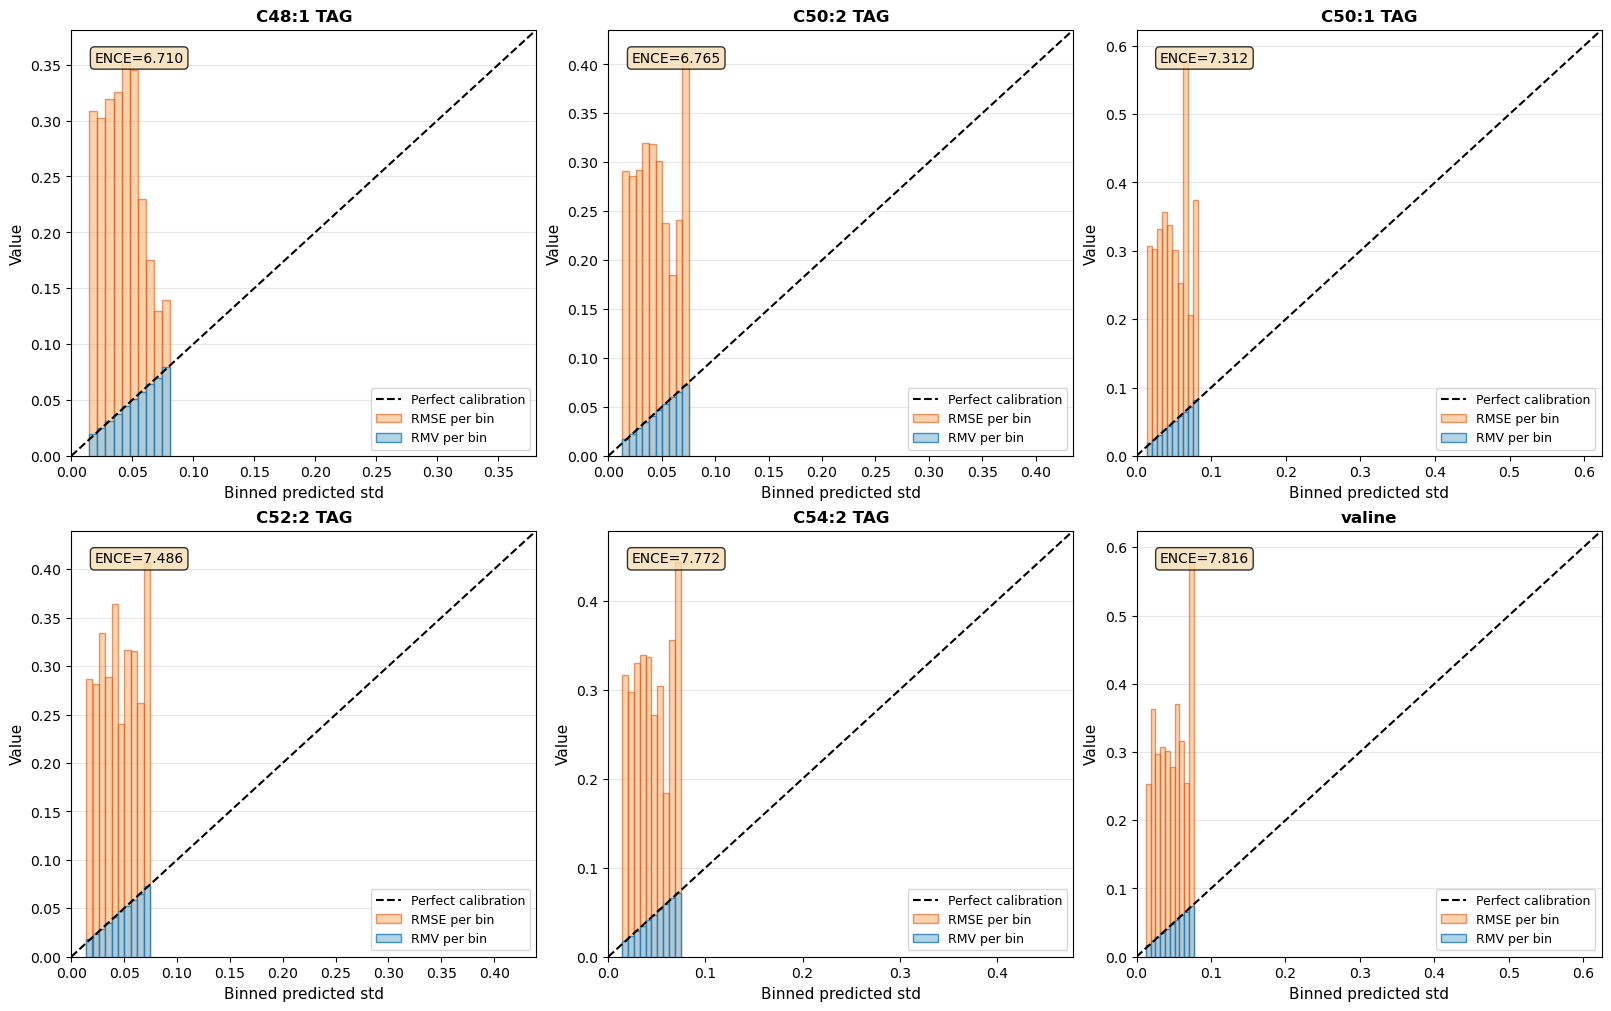
\includegraphics[width=\linewidth]{images/metabolomics_fig/metabolomics_calibration_curves_smallest_ece.png}
        \caption{Smallest calibration errors.}
        \label{fig:metabolomics_calibration_curves_smallest}
    \end{subfigure}
    \hfill
    \begin{subfigure}{0.48\linewidth}
        \centering
        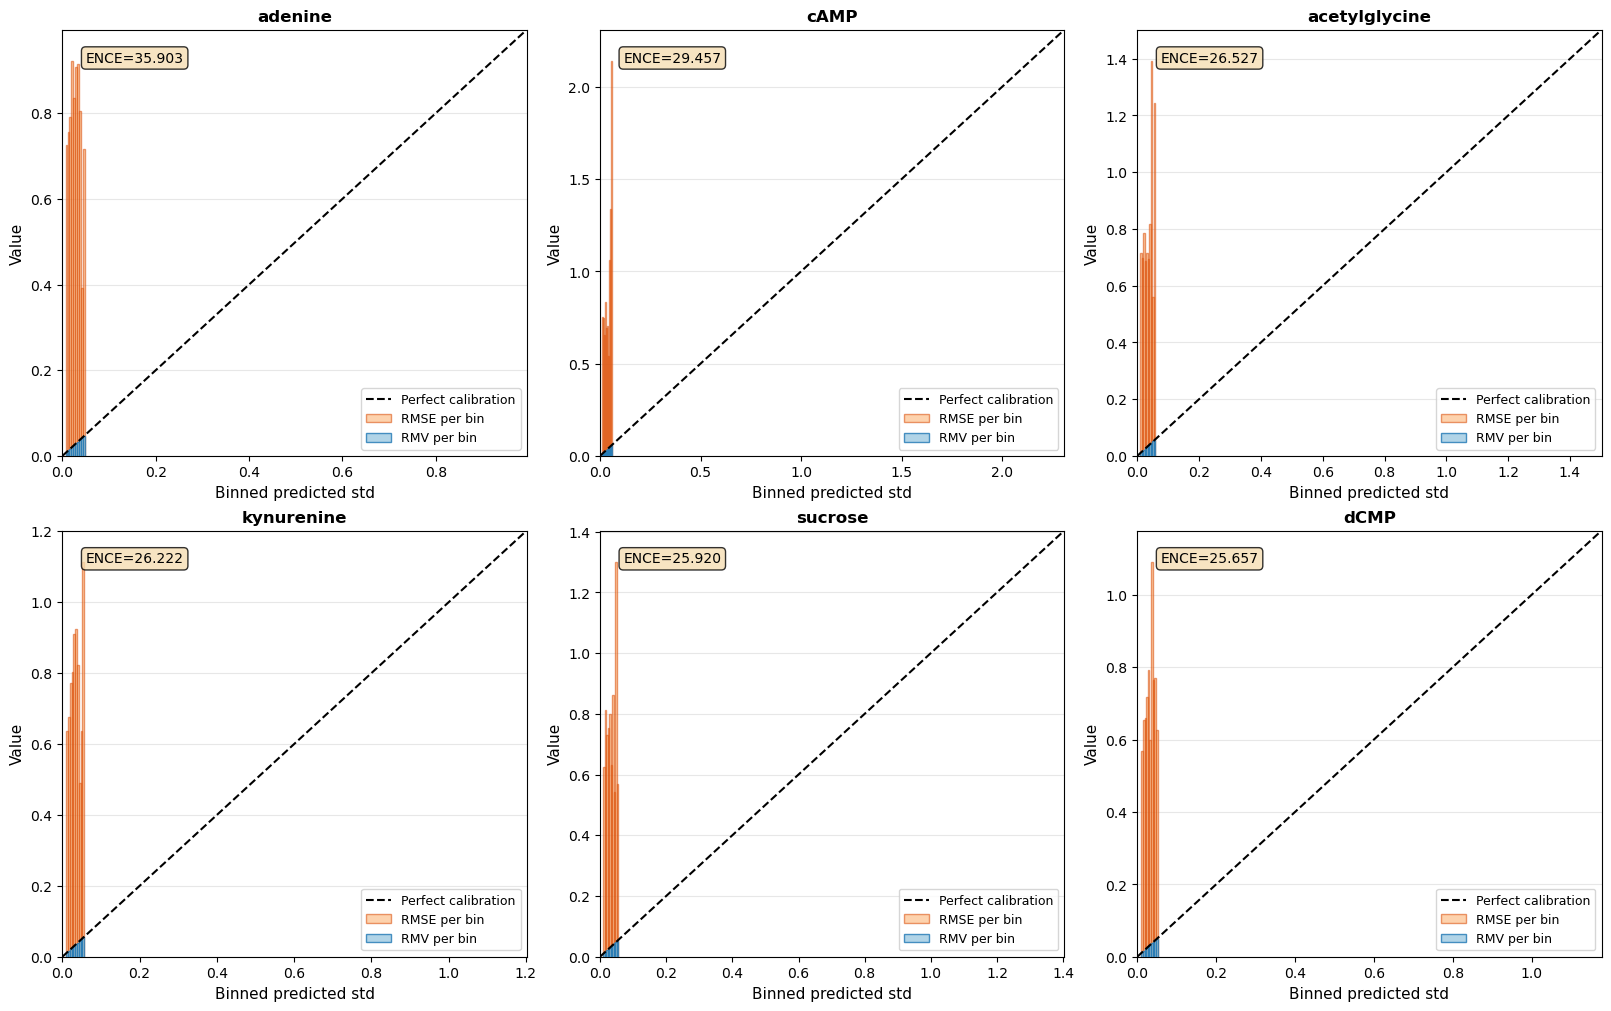
\includegraphics[width=\linewidth]{images/metabolomics_fig/metabolomics_calibration_curves_largest_ece.png}
        \caption{Largest calibration errors.}
        \label{fig:metabolomics_calibration_curves_largest}
    \end{subfigure}
    \caption[Metabolomics calibration curves]{Metabolomics calibration curves for the features with the smallest and largest calibration errors under Latent Space Sampling in-sample.}
    \label{fig:metabolomics_calibration_curves}
\end{figure}

\subsubsection{Analysis of the Proteomics Dataset}

Proteomics follows the same pattern as the previous omics. Its PIW ranges from 0.0477 to 0.0968 in-sample and from 0.249 to 0.509 out-of-sample, a widening comparable to that of Metabolomics and Methylation. ENCE is correspondingly reduced out-of-sample, ranging from 10.4 to 52.5 in-sample and from 2.51 to 21.3 out-of-sample, with every feature having a lower ENCE out-of-sample. As shown in Figure \ref{fig:proteomics_sharp_cal_scor}, features with higher ENCE again tend to have narrower prediction intervals, with an $R^2$ of 0.565 in-sample and 0.481 out-of-sample. Despite the calibration improvement, out-of-sample features have a higher CRPS overall, and Proteomics has the highest out-of-sample mean CRPS after CRISPR-Cas9, at 0.655.

\begin{figure}[!ht]
    \centering
    \begin{subfigure}{0.48\linewidth}
        \centering
        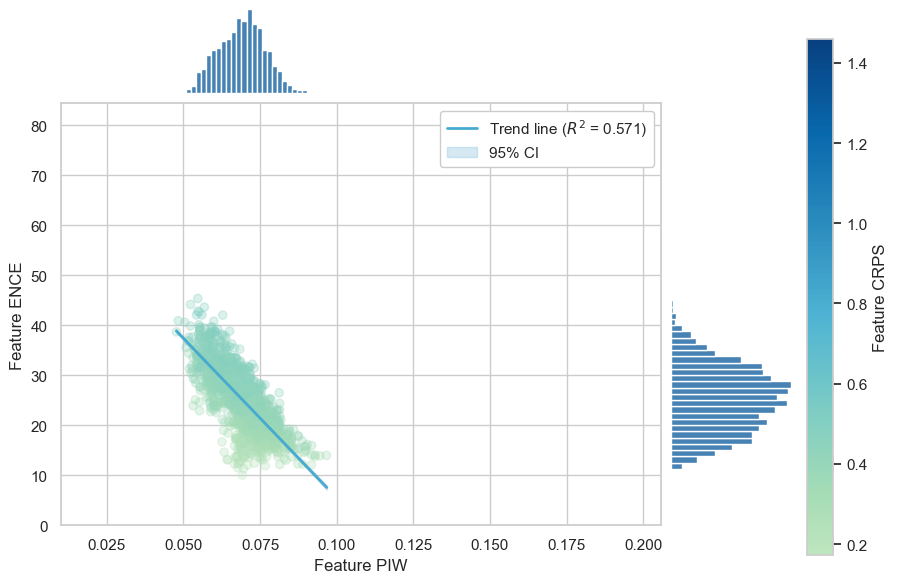
\includegraphics[width=\linewidth]{images/Proteomics/proteomics_sharp_cal_score_scaled.png}
        \caption{In-Sample data.}
        \label{fig:proteomics_sharp_cal_scor_in}
    \end{subfigure}
    \hfill
    \begin{subfigure}{0.48\linewidth}
        \centering
        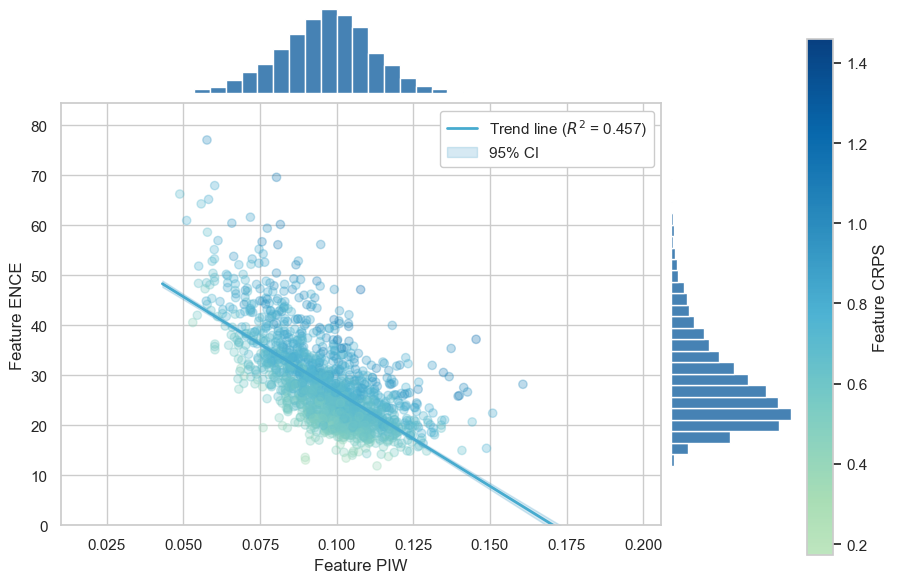
\includegraphics[width=\linewidth]{images/Proteomics/proteomics_sharp_cal_score_OOD_scaled.png}
        \caption{Out-of-Sample data.}
        \label{fig:proteomics_sharp_cal_scor_out}
    \end{subfigure}
    \caption[Proteomics PIW-ENCE scatter plots]{Proteomics feature-wise scatter plots between PIW and ENCE with CRPS value as a gradient.}
    \label{fig:proteomics_sharp_cal_scor}
\end{figure}

The correlation structure in Figure \ref{fig:corr_proteomics_metrics} clarifies two central aspects of Proteomics. First, the usual pattern between uncertainty and reconstruction quality remains present, as in-sample ENCE has a strong positive association with CRPS and RMSE and a strong negative association with feature correlation. The same holds out-of-sample, although more weakly for calibration, with ENCE correlating 0.795 with CRPS and 0.767 with RMSE. Proteomics also stands out because missingness appears to play a more important role than in the previous omics. The training data has a high mean missing-value rate of 47.9\%, with some features missing most of their observations. In both in-sample and out-of-sample data, missing values correlate negatively with PIW and positively with ENCE, CRPS and RMSE. These associations are strongest for PIW, at -0.75 in-sample and -0.76 out-of-sample, and for ENCE, at 0.672 and 0.630, indicating that features with more missing training data tend to be more miscalibrated and harder to reconstruct. These features also tend to have narrower intervals.

\begin{figure}[!ht]
    \centering
    \begin{subfigure}{0.48\linewidth}
        \centering
        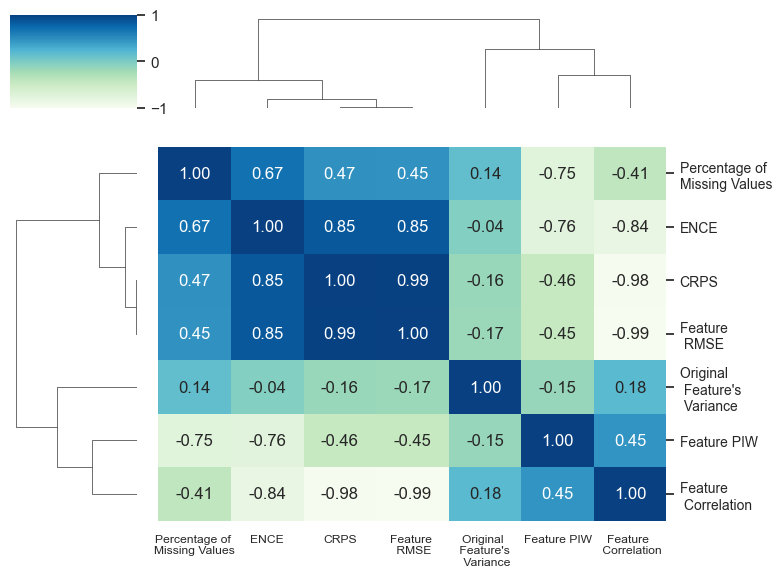
\includegraphics[width=\linewidth]{images/Proteomics/proteomics_cluster_map.png}
        \caption{In-Sample data.}
        \label{fig:corr_proteomics_metrics_in}
    \end{subfigure}
    \hfill
    \begin{subfigure}{0.48\linewidth}
        \centering
        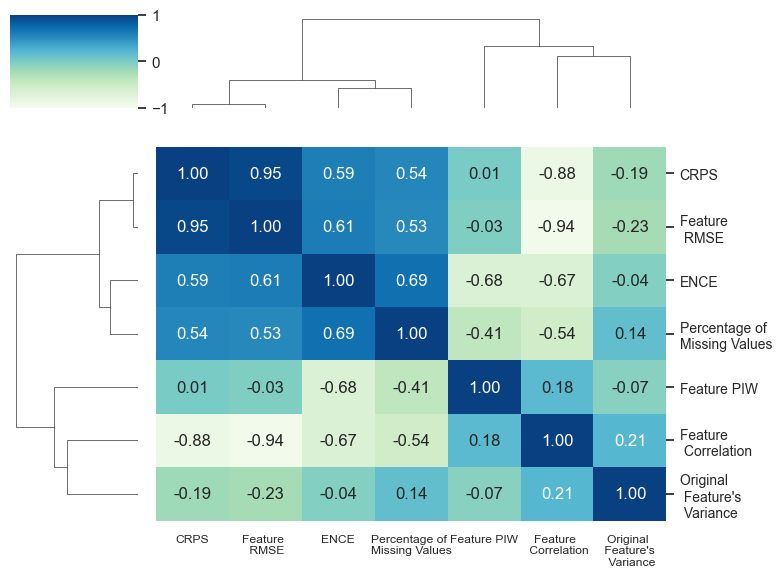
\includegraphics[width=\linewidth]{images/Proteomics/proteomics_cluster_map_OOD.png}
        \caption{Out-of-Sample data.}
        \label{fig:corr_proteomics_metrics_out}
    \end{subfigure}
    \caption[Proteomics uncertainty correlation cluster-map]{Pearson correlation cluster-map between feature-wise uncertainty metrics, reconstruction-error metrics, missing-value percentage and original feature variance for Proteomics.}
    \label{fig:corr_proteomics_metrics}
\end{figure}

This effect is seen more directly in Figure \ref{fig:proteomics_cal_rmse_miss} where, to highlight the role of missing data in calibration, the missingness percentage was used as a colour gradient. As in the previous omics, better reconstructed features tend to have lower ENCE values and this relationship is stronger for in-sample data, as 70\% of the variability of ENCE can be explained by RMSE. This is reflected in the $R^2$ of 0.707 for in-sample data and 0.588 for out-of-sample data. In-sample RMSE ranges from 0.245 to 0.744, while out-of-sample RMSE ranges from 0.430 to 1.77, again showing substantially worse reconstruction out-of-sample. Unlike the previous omics, however, the missing-value rate is visibly aligned with this pattern in both reconstructions. Features with higher ENCE also tend to have higher missingness, and in both plots the features with at least 50\% missing values lie above the main trend, with a higher ENCE than their RMSE alone would suggest. The sharpness and calibration values from Proteomics therefore support the broader conclusion that out-of-sample reconstructions are harder even when uncertainty estimates partially broaden.

\begin{figure}[!ht]
    \centering
    \begin{subfigure}{0.48\linewidth}
        \centering
        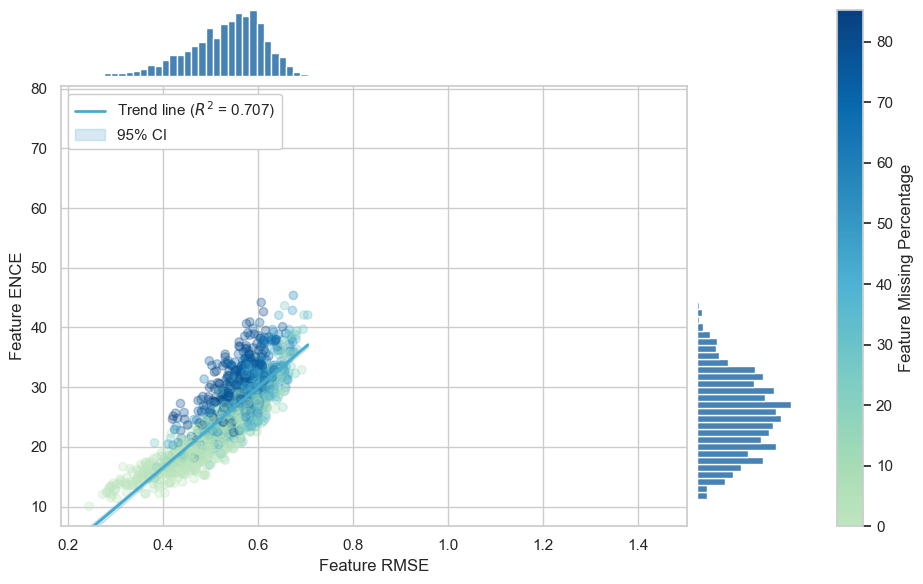
\includegraphics[width=\linewidth]{images/Proteomics/Proteomics_scor_rmse_miss_sampled.png}
        \caption{In-Sample data.}
        \label{fig:proteomics_cal_rmse_miss_in}
    \end{subfigure}
    \hfill
    \begin{subfigure}{0.48\linewidth}
        \centering
        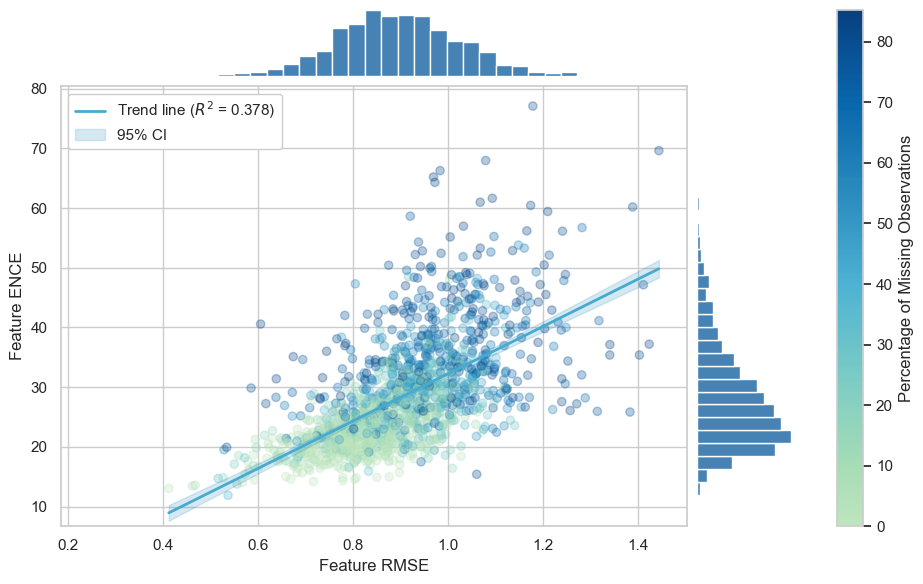
\includegraphics[width=\linewidth]{images/Proteomics/proteomics_scor_rmse_miss_OOD_scaled.png}
        \caption{Out-of-Sample data.}
        \label{fig:proteomics_cal_rmse_miss_out}
    \end{subfigure}
    \caption[Proteomics RMSE-ENCE scatter plots]{Proteomics feature-wise scatter plots between RMSE and ENCE, with missing values in the training data shown as a gradient.}
    \label{fig:proteomics_cal_rmse_miss}
\end{figure}

Proteomics therefore shows that the Metabolomics-like pattern also holds for a highly incomplete omic, with missingness contributing to the miscalibration of individual features. Transcriptomics and CRISPR-Cas9 also show sharp and poorly calibrated reconstructions, but their behaviour emphasises different aspects of the same problem. Transcriptomics has a strong in-sample association between ENCE and RMSE, at 0.81, that weakens out-of-sample, at 0.61, while CRISPR-Cas9 remains the sharpest and most miscalibrated continuous omic in both settings. In both cases, CRPS tracks RMSE more consistently than ENCE after the omic-specific input is removed, with out-of-sample correlations with RMSE of 0.86 and 0.79 for CRPS against 0.61 and 0.19 for ENCE, supporting the interpretation that scoring rules are more stable indicators of reconstruction difficulty in the out-of-sample setting.

\subsubsection{Analysis of the Copy number Dataset}

As previously mentioned, the uncertainty metrics used for the continuous datasets are replaced by categorical counterparts for Copy number. The entropy of the reconstruction samples was used for sharpness, ECE for calibration, Log Score as the scoring rule and balanced accuracy as the measure of reconstruction quality. Balanced accuracy is used because Copy number data is strongly imbalanced, as is common in biological datasets and when the original data is not diverse. Another measure used to better understand the model's uncertainty was the original feature's diversity. This was calculated by measuring the feature-wise normalised Shannon's entropy of the ground truth data. This value is therefore the same for both the in-sample and out-of-sample plots. This measure is referred to as feature diversity to prevent confusion with the entropy used as a sharpness metric.

Compared with the continuous omics, Copy number provides the categorical counterpart to the same uncertainty analysis. As with the continuous omics, Copy number shows very sharp reconstructions for all features. Mean feature entropy is close to zero for both in-sample and out-of-sample data, ranging from 0 to 0.0471 in-sample and from 0 to 0.0674 out-of-sample. Unlike the continuous datasets, however, this sharpness is not accompanied by uniformly severe miscalibration across all features. ECE ranges from imperfect calibration to clear miscalibration, with values between 0.109 and 0.631 in-sample and between 0.155 and 0.707 out-of-sample. Figure \ref{fig:copynumber_sharp_cal_scor} shows that, in-sample, sharper features are generally also better calibrated, with 52.3\% of ECE variability explained by the reconstruction entropy, as shown in Figure \ref{fig:copynumber_sharp_cal_scor_in}. Features with higher entropy and higher ECE also tend to have higher Log Score. This relationship becomes much weaker out-of-sample, where the corresponding $R^2$ is only 0.098 and features are generally more miscalibrated.

\begin{figure}[!ht]
    \centering
    \begin{subfigure}{0.48\linewidth}
        \centering
        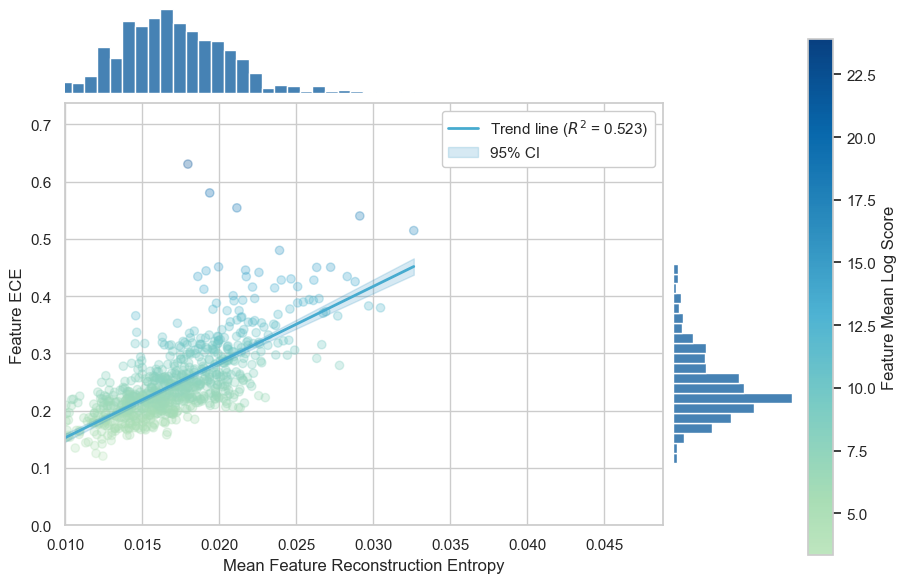
\includegraphics[width=\linewidth]{images/CopyNumber_fig/copynumber_sharp_cal_score_scaled_sample_hist.png}
        \caption{In-Sample data.}
        \label{fig:copynumber_sharp_cal_scor_in}
    \end{subfigure}
    \hfill
    \begin{subfigure}{0.48\linewidth}
        \centering
        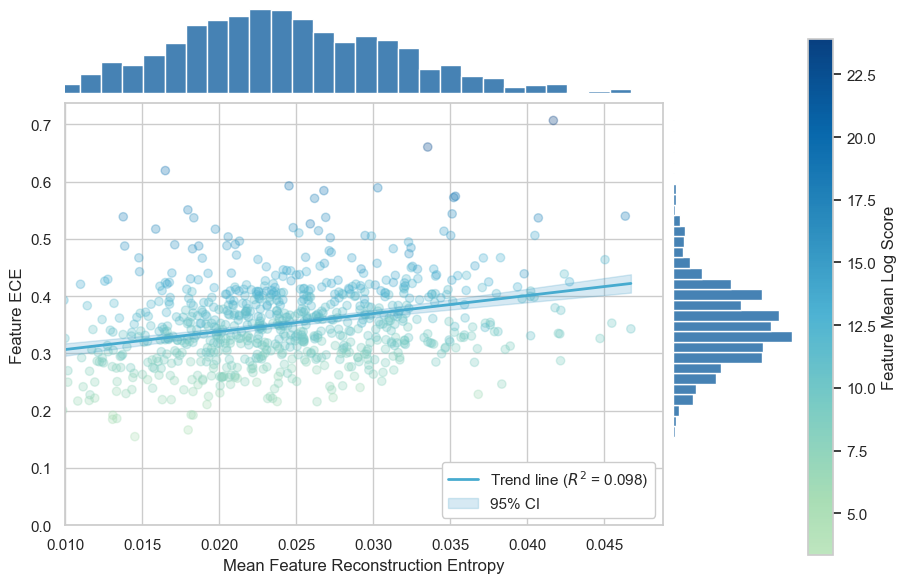
\includegraphics[width=\linewidth]{images/CopyNumber_fig/copynumber_sharp_cal_score_scaled_sample_hist_OOD.png}
        \caption{Out-of-Sample data.}
        \label{fig:copynumber_sharp_cal_scor_out}
    \end{subfigure}
    \caption[Copy number entropy-ECE scatter plots]{Copy number feature-wise scatter plots between entropy and ECE with Log Score value as a gradient.}
    \label{fig:copynumber_sharp_cal_scor}
\end{figure}

The correlation matrix cluster-maps in Figure \ref{fig:corr_copynumber_metrics} support these observations. In-sample, mean feature entropy is strongly positively correlated with ECE and moderately with Log Score, with correlations of 0.723 and 0.692 respectively, while balanced accuracy is negatively correlated with both ECE and Log Score. This indicates that sharper and better calibrated features are generally reconstructed more accurately. ECE and Log Score are almost perfectly correlated in both settings, showing that the scoring rule is strongly connected to calibration errors in the categorical reconstruction. Out-of-sample entropy has weak to moderate correlations with all other analysed metrics, of at most 0.36, while ECE remains strongly correlated with Log Score and moderately negatively correlated with balanced accuracy. Feature diversity is also moderately correlated with ECE and Log Score out-of-sample, with a higher correlation than for in-sample reconstructions. This suggests that the model is worse at estimating its certainty for features with more diverse class distributions without Copy number input.

\begin{figure}[!ht]
    \centering
    \begin{subfigure}{0.48\linewidth}
        \centering
        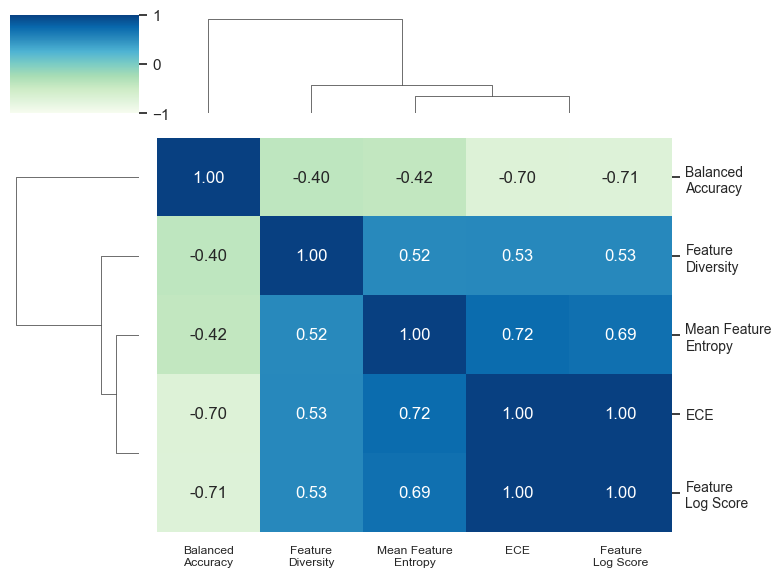
\includegraphics[width=\linewidth]{images/CopyNumber_fig/copynumber_cluster_map.png}
        \caption{In-Sample data.}
        \label{fig:corr_copynumber_metrics_in}
    \end{subfigure}
    \hfill
    \begin{subfigure}{0.48\linewidth}
        \centering
        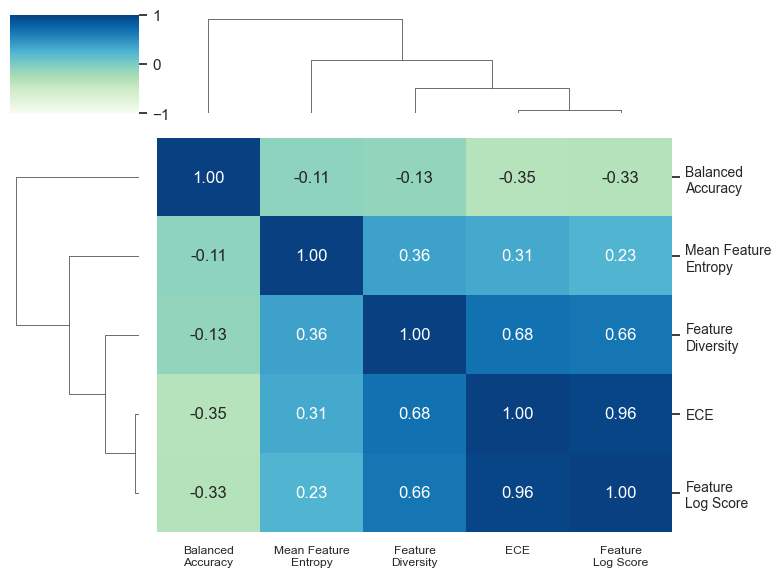
\includegraphics[width=\linewidth]{images/CopyNumber_fig/copynumber_cluster_map_OOD.png}
        \caption{Out-of-Sample data.}
        \label{fig:corr_copynumber_metrics_out}
    \end{subfigure}
    \caption[Copy number uncertainty correlation cluster-maps]{Pearson correlation cluster-map between the measures used to analyse uncertainty in Copy number.}
    \label{fig:corr_copynumber_metrics}
\end{figure}

Figure \ref{fig:copynumber_ece_acc_entropy} further compares calibration with reconstruction quality. In-sample data shows that better calibrated features are again associated with better reconstruction quality, with an $R^2$ of 0.494 between ECE and balanced accuracy. Out-of-sample, balanced accuracy decreases and the points become more dispersed, so the same trend is much weaker, with an $R^2$ of 0.122. The relationship between feature diversity and feature ECE previously mentioned can also be seen through the data point colour gradient.

\begin{figure}[!ht]
    \centering
    \begin{subfigure}{0.48\linewidth}
        \centering
        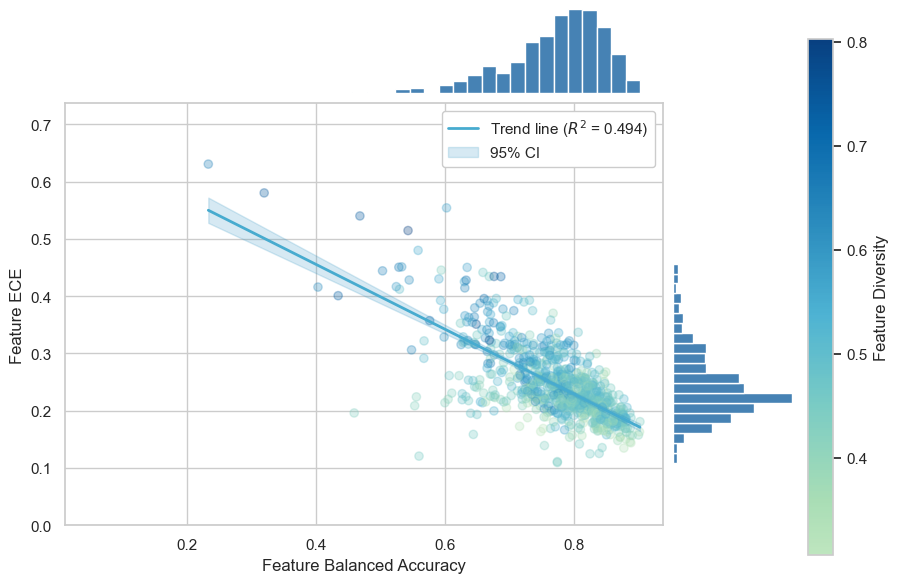
\includegraphics[width=\linewidth]{images/CopyNumber_fig/copynumber_ECE_acc_entropy.png}
        \caption{In-Sample data.}
        \label{fig:copynumber_ece_acc_entropy_in}
    \end{subfigure}
    \hfill
    \begin{subfigure}{0.48\linewidth}
        \centering
        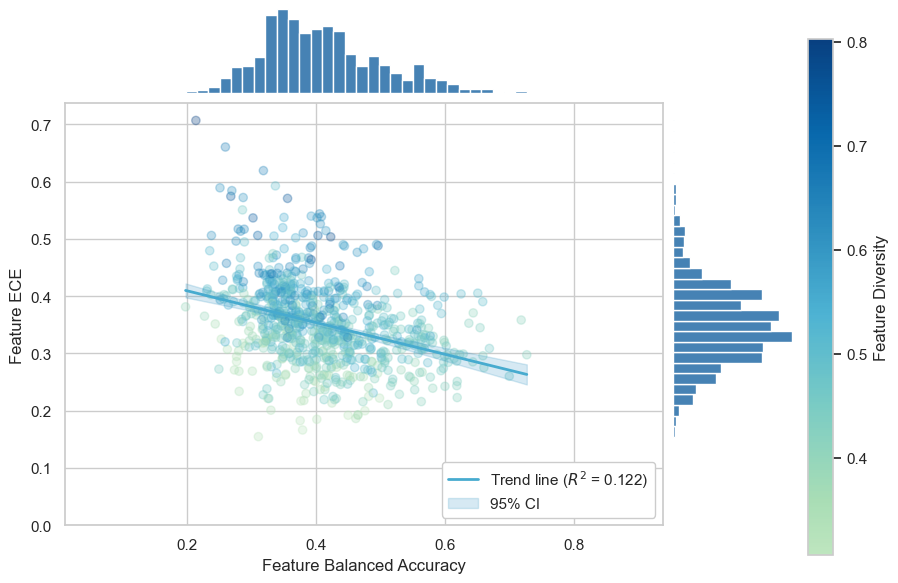
\includegraphics[width=\linewidth]{images/CopyNumber_fig/copynumber_ECE_acc_entropy_OOD.png}
        \caption{Out-of-Sample data.}
        \label{fig:copynumber_ece_acc_entropy_out}
    \end{subfigure}
    \caption[Copy number accuracy-ECE scatter plots]{Copy number feature-wise scatter plots between balanced accuracy and ECE with ground truth entropy as a gradient.}
    \label{fig:copynumber_ece_acc_entropy}
\end{figure}

Looking more closely at individual classes, Figure \ref{fig:copynumber_sharpness_per_original_class} shows the reconstruction sharpness of each class, together with data points with missing values. This class-wise summary was obtained using the following pseudo-code.

\begin{figure}[!ht]
\centering
\fbox{%
\begin{minipage}{0.92\linewidth}
\textbf{Algorithm} Class-wise mean Copy number sharpness calculation

\textbf{Input:} Original Copy number matrix $X^{\mathrm{true}}$, reconstruction sharpness matrix $H^{\mathrm{recon}}$ \\
\textbf{Output:} Mean reconstruction entropy $\bar{H}_{c}$ for each class

\begin{tabular}{ll}
1: & \textbf{for each} $c \in \{-2,-1,0,1,2,\mathrm{NA}\}$ \textbf{do} \\
2: & \quad $\mathcal{I}_{c} \leftarrow \{(i,j) : X_{ij}^{\mathrm{true}} = c\}$ \\
3: & \quad $H_{c} \leftarrow \{H_{ij}^{\mathrm{recon}} : (i,j) \in \mathcal{I}_{c}\}$ \\
4: & \quad $\bar{H}_{c} \leftarrow \frac{1}{|\mathcal{I}_{c}|}\sum_{(i,j) \in \mathcal{I}_{c}} H_{ij}^{\mathrm{recon}}$ \\
5: & \textbf{end for} \\
6: & \textbf{return} $\{\bar{H}_{c}\}_{c \in \{-2,-1,0,1,2,\mathrm{NA}\}}$
\end{tabular}
\end{minipage}%
}
\caption[Class-wise Copy number sharpness calculation algorithm]{Algorithm used to compute class-wise mean Copy number sharpness by grouping reconstructed entropy values according to the corresponding true class.}
\label{fig:copy_number_classwise_sharpness_algorithm}
\end{figure}

Here, $X_{ij}^{\mathrm{true}}$ denotes the original class for a Copy number observation $i$ and feature $j$, while $H_{ij}^{\mathrm{recon}}$ denotes the sharpness of the corresponding reconstructed data point.

For all five observed classes, out-of-sample reconstructions are less sharp than in-sample reconstructions. Missing-value reconstructions, however, show very similar sharpness in both settings. Class $-2$ is particularly notable, as it has the sharpest in-sample data points while having the highest out-of-sample entropy among the five classes. This likely reflects its very low representation in the original data, where it accounts for 0.4\% of total data points. By contrast, class $2$ is also rare, representing only 1.77\% of the data, but does not show the same large in-sample to out-of-sample deviation. Along with balanced accuracy in Figure \ref{fig:copynumber_ece_acc_entropy}, this is consistent with the model overfitting the Copy number dataset, which leads to less certainty in the reconstruction of out-of-sample data. Despite this, even for out-of-sample data, the model has very sharp predictions.

\begin{figure}[!ht]
    \centering
    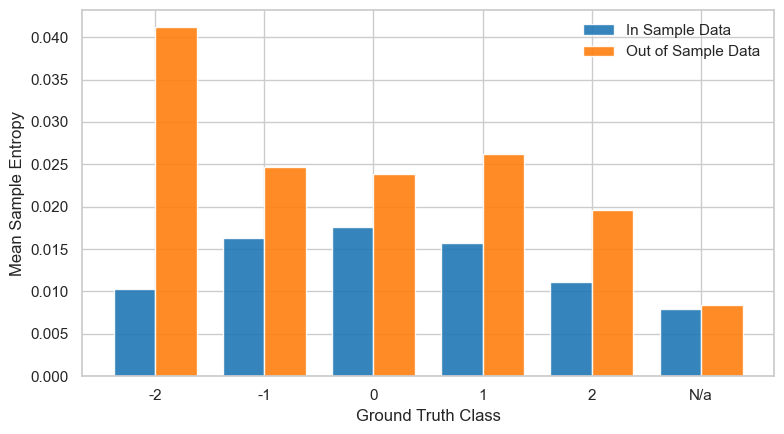
\includegraphics[width=0.75\linewidth]{images/CopyNumber_fig/sharpness_per_original_class.png}
    \caption[Copy number sharpness by class bar plot]{Copy number sharpness bar plot by original class divided by in-sample and out-of-sample.}
    \label{fig:copynumber_sharpness_per_original_class}
\end{figure}


\section{Monte Carlo Dropout} \label{chapter:MCD_analysis}

This section follows a structure similar to the previous Latent Space Sampling analysis, but focuses on uncertainty estimated from the Monte Carlo Dropout method described in Section \ref{Monte_Carlo_Dropout}. Instead of sampling \gls{MOSA}'s latent representation and decoding the resulting latent vectors, Monte Carlo Dropout keeps dropout active during inference and repeatedly forwards the same input through the model. The resulting set of reconstructions therefore captures variability induced by different active subnetworks of the trained model.

This distinction changes the interpretation of the uncertainty being analysed. While the previously analysed method focused on aleatoric uncertainty encoded in the VAE's latent representation, Monte Carlo Dropout is used here as an approximation of epistemic uncertainty. In this context, the variability between reconstructions reflects uncertainty related to the model itself. This includes uncertainty about the learned parameterisation and about which parts of the network are most reliable for a given input. This makes both analyses complementary. While Section \ref{LSS_Analysis} describes uncertainty intrinsic to the decoded data distribution, Monte Carlo Dropout evaluates how stable the model's predictions are under stochastic changes to the network during inference.

As before, the analysis is performed across the seven reconstructed omics and compares in-sample with out-of-sample reconstructions.

As will be discussed during the analysis, an issue arises in the out-of-sample Monte Carlo Dropout reconstructions of Methylation and CRISPR-Cas9. For several features, a non-negligible fraction of data points has predictive variance \(\sigma^2(x_i)\) equal or very close to zero. Since ENCE bins predictions by their predicted uncertainty and compares the root mean squared error, \(\mathrm{RMSE}(b)\), with the root mean variance, \(\mathrm{RMV}(b)\), each bin contributes a normalised term of the form \(|\mathrm{RMSE}(b)-\mathrm{RMV}(b)|/\mathrm{RMV}(b)\). When \(\mathrm{RMV}(b)\) is close to zero, but the reconstruction error remains positive, this ratio can become extremely large. These near-zero variances follow from how the Monte Carlo Dropout outputs are stored. In the original MOSA implementation, the predicted means and variances are saved rounded to five decimal places. Since most out-of-sample Methylation and CRISPR-Cas9 variances are of the order of $10^{-5}$, the smallest of them are stored as exactly zero. For Methylation, 94\% of the out-of-sample variances are below $10^{-4}$ and 40\% are equal to zero. These cases therefore correspond to features where the model has close to zero uncertainty while still making reconstruction errors, meaning that ENCE correctly identifies them as strongly overconfident.

This behaviour is taken into consideration in the interpretation of the Monte Carlo Dropout results. However, to keep the summary plots and tables readable, out-of-sample features with ENCE larger than \(10^3\) are excluded from the visual and tabular summaries in this section. This filtering removes 8,273 out-of-sample Methylation features and 2,286 out-of-sample CRISPR-Cas9 features, 57\% and 13\% of the features of the two omics. No feature has an ENCE between 37 and 2,000, so the exact threshold does not change which features are excluded. The exclusion is therefore only a visualisation and summarisation choice; analytically, these removed features remain important for the following analysis.

%These features also tend to be those for which more than 5\% of the data points have zero predictive variance.
%Será que tem haver com um filtering feito antes do treino do modelo em que se remove as features com menos variabilidade? Ver isto


%\subsection{General Analysis}
\subsection{Analysis of Uncertainty at the Dataset Level}

The Monte Carlo Dropout results show a clear contrast of the uncertainty profile from the Latent Space Sampling analysis, both in terms of range of values sampled, as well as the distribution of these values.

At the dataset level, the most easily identifiable pattern is that all continuous omics have lower mean PIW out-of-sample than in-sample. This is the opposite of what would usually be expected as missing an omic-specific input should make the model less certain and thus less sharp. Metabolomics decreases from an in-sample mean PIW of 3.94 to 0.670 out-of-sample, Methylation decreases from 5.68 to 0.112, and CRISPR-Cas9 decreases from 4.80 to 0.235. The same direction is observed for Drug Response, Proteomics and Transcriptomics, although with smaller absolute differences. Here, when the omic-specific input is removed the dropout-affected reconstructions lead to more stable, lower-variance predictions. Feature predictions shift toward a common reconstruction across dropout masks, creating sharper predictive distributions for out-of-sample data.


The standard deviations displayed in Table \ref{tab:uncertainty_summary_all_metrics_sideways_MCD} show that this behaviour is not uniform across all features. The largest in-sample PIW standard deviations occur for Methylation, Metabolomics, and CRISPR-Cas9. These three omics are also the ones that stand out most clearly in Figure \ref{fig:mcd_sharpness_features_piw}, where their feature-wise PIW distributions are much wider than the remaining continuous datasets. Methylation is the most extreme case, with some features having mean PIW larger than 10. 

\begin{figure}[!ht]
    \centering
    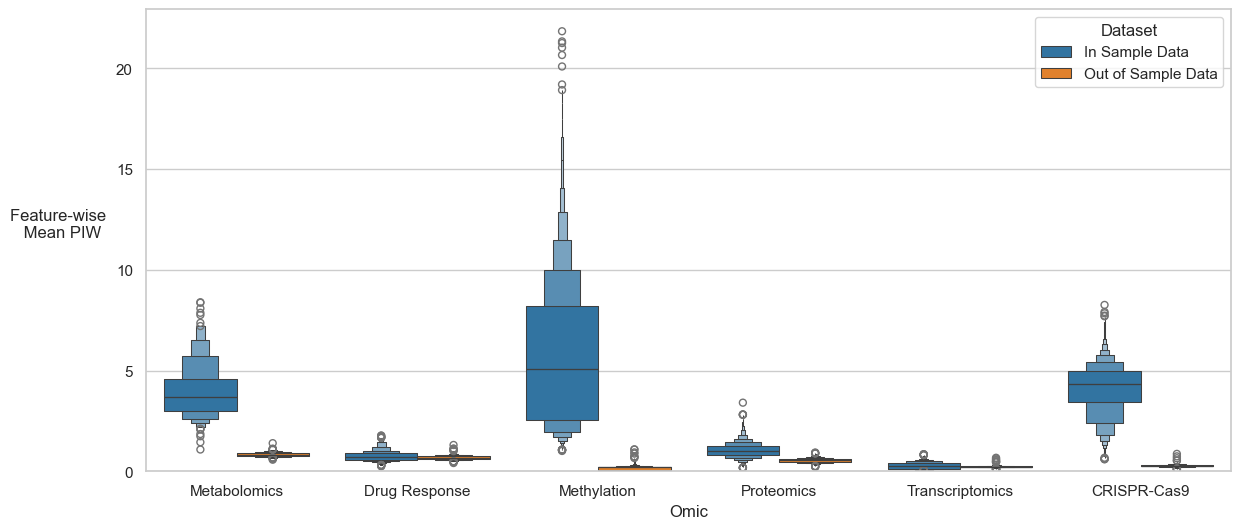
\includegraphics[width=0.9\linewidth]{images/MCD/Sharpness_features_PIW_MCD.png}
    \caption[MCD continuous omic sharpness boxen plots]{Boxen plot of feature-wise mean PIW calculated from Monte Carlo Dropout samples for the continuous omic datasets.}
    \label{fig:mcd_sharpness_features_piw}
\end{figure}

\begin{landscape}
\begin{table}[p]
\centering
\begin{tabular}{|c|cccc|cccc|cccc|}
\hline
\multirow{3}{*}{Dataset} & \multicolumn{4}{c|}{Sharpness}                                              & \multicolumn{4}{c|}{Calibration}                                           & \multicolumn{4}{c|}{Scoring Rules}                                         \\ \cline{2-13}
                         & \multicolumn{2}{c|}{In-Sample}         & \multicolumn{2}{c|}{Out-of-Sample} & \multicolumn{2}{c|}{In-Sample}        & \multicolumn{2}{c|}{Out-of-Sample} & \multicolumn{2}{c|}{In-Sample}         & \multicolumn{2}{c|}{Out-of-Sample} \\ \cline{2-13}
                         & $\mu$  & \multicolumn{1}{c|}{$\sigma$} & $\mu$           & $\sigma$         & $\mu$ & \multicolumn{1}{c|}{$\sigma$} & $\mu$          & $\sigma$          & $\mu$  & \multicolumn{1}{c|}{$\sigma$} & $\mu$          & $\sigma$         \\ \hline
Metabolomics             & 3.94 & \multicolumn{1}{c|}{1.37} & 0.670 & 0.0612 & 0.560 & \multicolumn{1}{c|}{0.111} & 3.73 & 0.770 & 0.359 & \multicolumn{1}{c|}{0.0798} & 0.611 & 0.0830 \\
Drug Response            & 0.747 & \multicolumn{1}{c|}{0.266} & 0.568 & 0.0588 & 1.77 & \multicolumn{1}{c|}{0.759} & 4.16 & 0.785 & 0.330 & \multicolumn{1}{c|}{0.0508} & 0.569 & 0.0837 \\
Methylation\textsuperscript{*}              & 5.68 & \multicolumn{1}{c|}{3.46} & 0.112 & 0.0769 & 0.568 & \multicolumn{1}{c|}{0.198} & 14.2 & 2.56 & 0.475 & \multicolumn{1}{c|}{0.166} & 0.567 & 0.0813 \\
Proteomics               & 1.05 & \multicolumn{1}{c|}{0.367} & 0.400 & 0.0546 & 1.33 & \multicolumn{1}{c|}{0.882} & 6.99 & 1.81 & 0.317 & \multicolumn{1}{c|}{0.0514} & 0.643 & 0.114 \\
Transcriptomics          & 0.315 & \multicolumn{1}{c|}{0.202} & 0.173 & 0.0114 & 9.56 & \multicolumn{1}{c|}{7.18} & 15.4 & 2.85 & 0.420 & \multicolumn{1}{c|}{0.0603} & 0.606 & 0.0904 \\
CRISPR-Cas9\textsuperscript{*}              & 4.80 & \multicolumn{1}{c|}{1.43} & 0.235 & 0.0159 & 0.522 & \multicolumn{1}{c|}{0.125} & 14.1 & 2.68 & 0.479 & \multicolumn{1}{c|}{0.0533} & 0.757 & 0.0998 \\ \hline
\end{tabular}
\begin{center}
\footnotesize \textsuperscript{*}The out-of-sample Methylation and CRISPR-Cas9 ENCE values presented in this table were calculated after the feature exclusion outlined in Section \ref{chapter:MCD_analysis}.
\end{center}
\caption{Summary table of uncertainty metrics obtained from Monte Carlo Dropout for continuous datasets, split by in-sample and out-of-sample subsets.}
\label{tab:uncertainty_summary_all_metrics_sideways_MCD}
\end{table}
\end{landscape}

\begin{table}
\centering
\resizebox{\textwidth}{!}{%
\begin{tabular}{|c|cccc|cccc|cccc|}
\hline
\multirow{3}{*}{Dataset} & \multicolumn{4}{c|}{Sharpness}                                              & \multicolumn{4}{c|}{Calibration}                                           & \multicolumn{4}{c|}{Scoring Rules}                                         \\ \cline{2-13}
                         & \multicolumn{2}{c|}{In-Sample}         & \multicolumn{2}{c|}{Out-of-Sample} & \multicolumn{2}{c|}{In-Sample}        & \multicolumn{2}{c|}{Out-of-Sample} & \multicolumn{2}{c|}{In-Sample}         & \multicolumn{2}{c|}{Out-of-Sample} \\ \cline{2-13}
                         & $\mu$  & \multicolumn{1}{c|}{$\sigma$} & $\mu$           & $\sigma$         & $\mu$ & \multicolumn{1}{c|}{$\sigma$} & $\mu$          & $\sigma$          & $\mu$  & \multicolumn{1}{c|}{$\sigma$} & $\mu$          & $\sigma$         \\ \hline
Copy number              & 0.265 & \multicolumn{1}{c|}{0.0537} & 0.158 & 0.0345 & 0.0767 & \multicolumn{1}{c|}{0.0439} & 0.264 & 0.0631 & 1.31 & \multicolumn{1}{c|}{0.890} & 5.15 & 1.61 \\ \hline
\end{tabular}%
}
\caption{Summary table of uncertainty metrics obtained from Monte Carlo Dropout for Copy number, split by in-sample and out-of-sample subsets.}
\label{tab:uncertainty_summary_copy_number_MCD}
\end{table}



For Copy number, the feature-wise mean entropy is uniformly low, with all values below 0.4, as shown in Figure~\ref{fig:mcd_copynumber_entropy}. It has a mean of 0.265 in-sample and 0.158 out-of-sample, as described in Table~\ref{tab:uncertainty_summary_copy_number_MCD}. The predicted categorical probability for Copy number features tends to be concentrated on a single class rather than spread across the remaining four classes. The out-of-sample decrease in mean entropy therefore indicates even more concentrated class probabilities out-of-sample.

\begin{figure}[!ht]
    \centering
    \begin{subfigure}{0.32\linewidth}
        \centering
        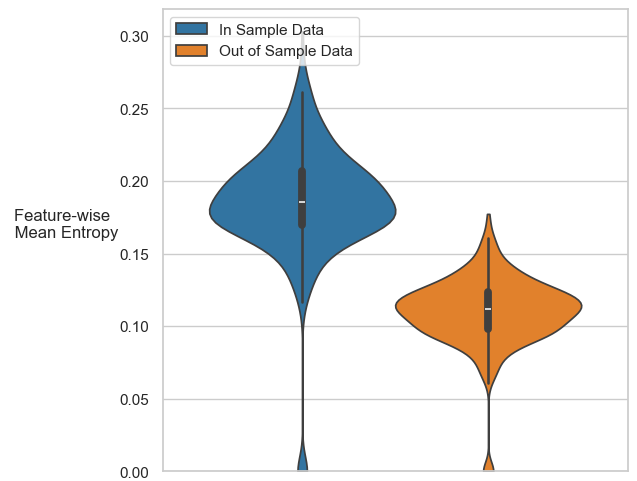
\includegraphics[width=\linewidth]{images/MCD/mcd_copynumber/copynumber_entropy_violin.png}
        \caption{Entropy.}
        \label{fig:mcd_copynumber_entropy}
    \end{subfigure}
    \hfill
    \begin{subfigure}{0.32\linewidth}
        \centering
        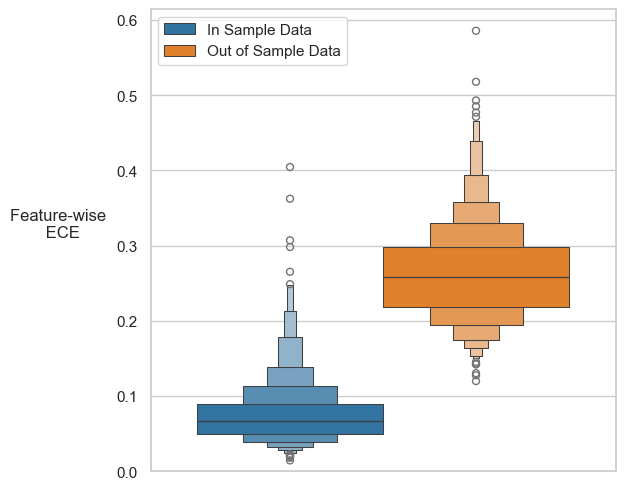
\includegraphics[width=\linewidth]{images/MCD/mcd_copynumber/copynumber_ECE.png}
        \caption{ECE.}
        \label{fig:mcd_copynumber_ece}
    \end{subfigure}
    \hfill
    \begin{subfigure}{0.32\linewidth}
        \centering
        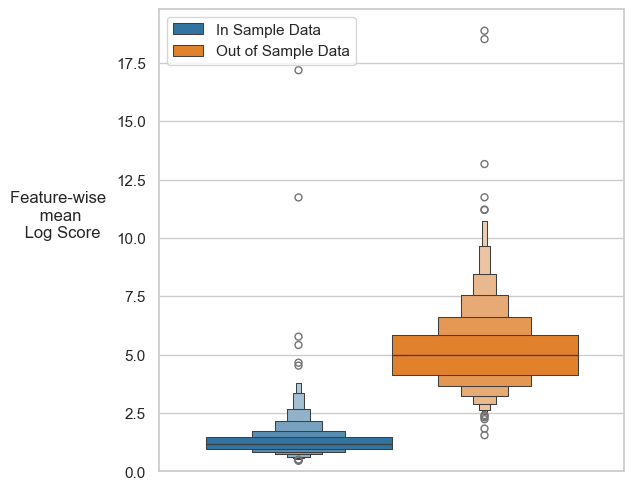
\includegraphics[width=\linewidth]{images/MCD/mcd_copynumber/copynumber_logscore.png}
        \caption{Log Score.}
        \label{fig:mcd_copynumber_logscore}
    \end{subfigure}
    \caption[MCD Copy number uncertainty metric plots]{Copy number uncertainty metrics calculated from Monte Carlo Dropout samples.}
    \label{fig:mcd_copynumber_metrics}
\end{figure}

%%%% Tenho também o violin plot destas figuras no folder images/MCD/mcd_copynumber.
%% Não mudei porque acho que os boxen plots com os outliers ficam visualmente mais apelativos sem perda substantiva de informação.

The calibration results provide the main evidence that the sharpness observed above is often not appropriate. In-sample Metabolomics, Methylation and CRISPR-Cas9 contain many features ranging from well calibrated to moderately miscalibrated. The features closer to 0 are more aligned with the empirical reconstruction error, both when compared with the remaining features in their dataset and with the values explored in Section \ref{LSS_Analysis}.

Drug Response has a mean ENCE of 1.77 and Proteomics has a mean of 1.33, both having features with ENCE values under 0.4 for Drug Response and 0.2 for Proteomics. Transcriptomics, unlike the remaining omics, has an in-sample mean ENCE of 9.56 and a standard deviation of 7.18. Its feature-wise ENCE ranges from 1.11 to 45.5.

Out-of-sample calibration error is higher for the continuous datasets. Metabolomics, Drug Response and Proteomics have the lowest out-of-sample ENCE means among the continuous omics, but these values still indicate clear miscalibration. Transcriptomics, Methylation and CRISPR-Cas9 have the highest out-of-sample mean ENCE values, at 15.4, 14.2 and 14.1 respectively, with the Methylation and CRISPR-Cas9 values calculated after excluding the previously mentioned extreme features. The increase observed when comparing the in-sample to the out-of-sample reconstructions is more prominent for Methylation and CRISPR-Cas9. These two datasets, other than Metabolomics, had the lowest ENCE values in-sample. Their out-of-sample results show that the model becomes overconfident when those omic inputs are missing.

The previously mentioned excluded out-of-sample features from Methylation and CRISPR-Cas9 reinforce this conclusion. The removed Methylation features have ENCE values ranging from \(2.04 \times 10^3\) to \(7.04 \times 10^8\), while the removed CRISPR-Cas9 features range from \(1.29 \times 10^4\) to \(1.40 \times 10^{11}\). These values identify features for which the Monte Carlo Dropout samples assign uncertainty close to zero, despite non-zero reconstruction error, and their magnitude follows from the variances stored as zero or close to zero. While the retained features in Figure \ref{fig:mcd_calibration_features_piw} already show out-of-sample miscalibration, the omitted features correspond to a more pronounced example of the overall pattern of out-of-sample miscalibration due to model overconfidence.

\begin{figure}[!ht]
    \centering
    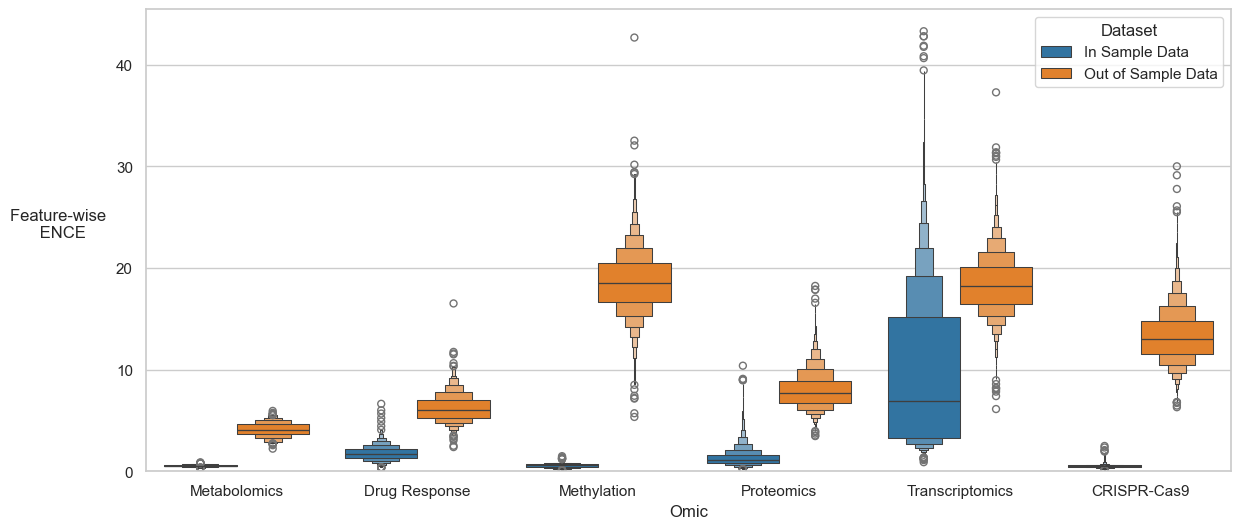
\includegraphics[width=0.9\linewidth]{images/MCD/ENCE_features_CRPS_MCD_snipped.png}
    \caption[MCD continuous omic calibration boxen plots]{Boxen plot of feature-wise ENCE calculated from Monte Carlo Dropout samples for the continuous omic datasets, with extreme values removed from the out-of-sample Methylation and CRISPR-Cas9 datasets.}
    \label{fig:mcd_calibration_features_piw}
\end{figure}

Copy number differs from the continuous omic datasets, with all feature-wise ECE values being below 0.6 for both in-sample and out-of-sample data, as seen in Figure \ref{fig:mcd_copynumber_ece}. The predicted categorical confidence is adjusted to the empirical accuracy of the predicted classes, although the out-of-sample setting still makes the class probabilities less reliable.

For all datasets, the mean scoring values are lower in-sample than out-of-sample. This consistent increase confirms that the out-of-sample uncertainty estimation of the reconstructions is worse, even when their sharpness values are lower. As previously concluded, the model is not improving by becoming sharper out-of-sample; it is producing narrower distributions that score worse due to being less aligned with the observed data.

\begin{figure}[!ht]
    \centering
    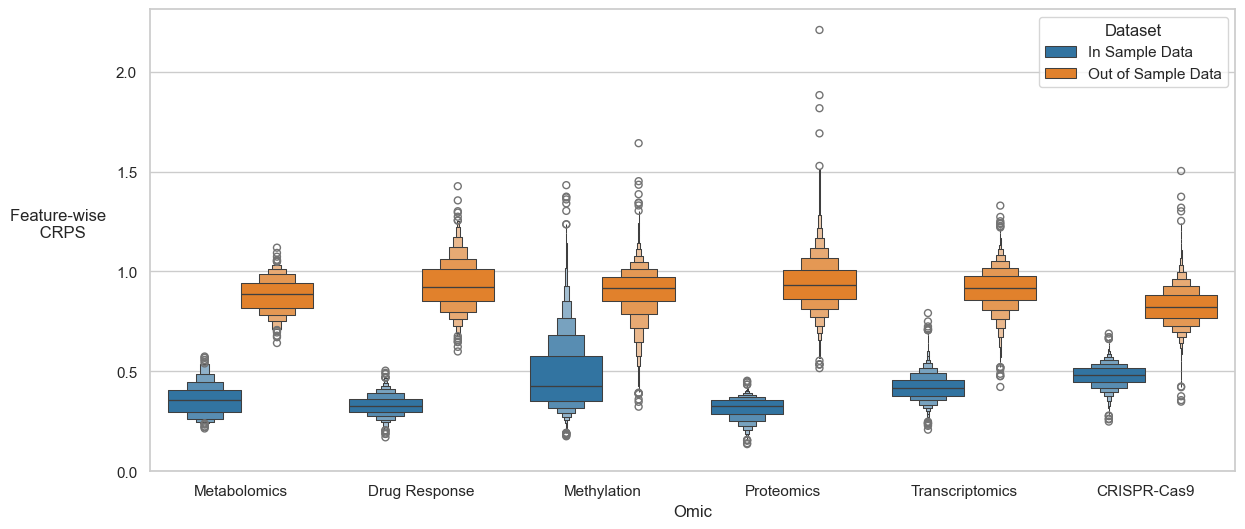
\includegraphics[width=0.9\linewidth]{images/MCD/Scoring_features_CRPS_MCD.png}
    \caption[MCD continuous omic scoring boxen plots]{Boxen plot of feature-wise mean CRPS calculated from Monte Carlo Dropout samples for the continuous omic datasets.}
    \label{fig:mcd_scoring_features_crps}
\end{figure}

\subsection{Analysis of Methylation and Proteomics}

The following analysis looks more closely at Methylation and Proteomics. These datasets were selected to illustrate two different behaviours observed in the Monte Carlo Dropout results. Methylation represents the more extreme overconfidence pattern, with broad in-sample predictive intervals but sharp out-of-sample intervals. Proteomics serves as a comparison as its behaviour is closer to the general out-of-sample trend shared by the continuous omics.

\subsubsection{Methylation}

Methylation shows the most extreme in-sample sharpness profile among the continuous omics. As seen in Figure \ref{fig:mcd_sharpness_features_piw}, its in-sample PIW is substantially larger than that of most other omics, and is only comparable to Metabolomics and CRISPR-Cas9, which also show a wider spread of feature-wise PIW values. This indicates that, when the Methylation input is available, different dropout subnetworks often produce substantially different reconstructions for the same features.

\begin{figure}[!ht]
    \centering
    \begin{subfigure}{0.48\linewidth}
        \centering
        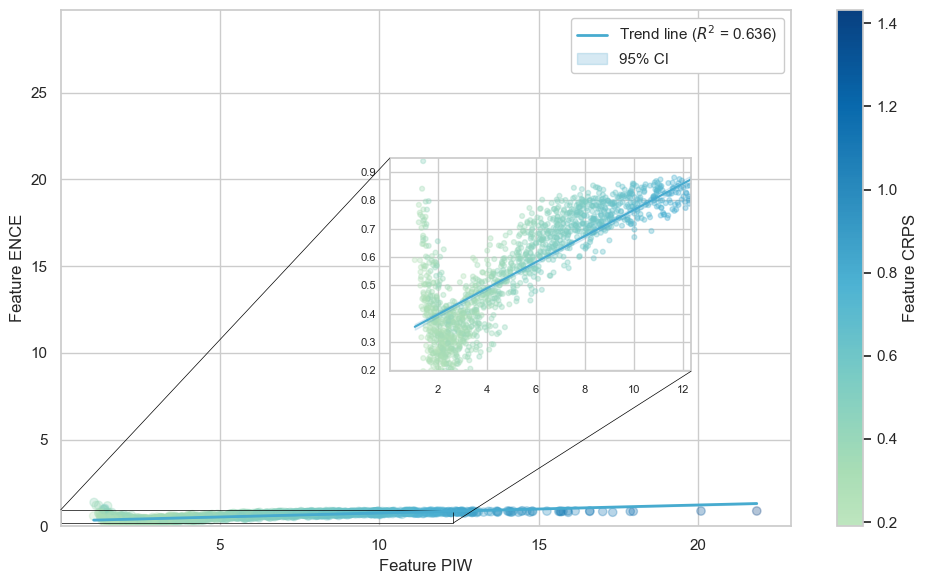
\includegraphics[width=\linewidth]{images/MCD/mcd_methylation/methyl_scatter_piw_ence_zoom.png}
        \caption{In-Sample data.}
        \label{fig:mcd_methylation_piw_ence_in}
    \end{subfigure}
    \hfill
    \begin{subfigure}{0.48\linewidth}
        \centering
        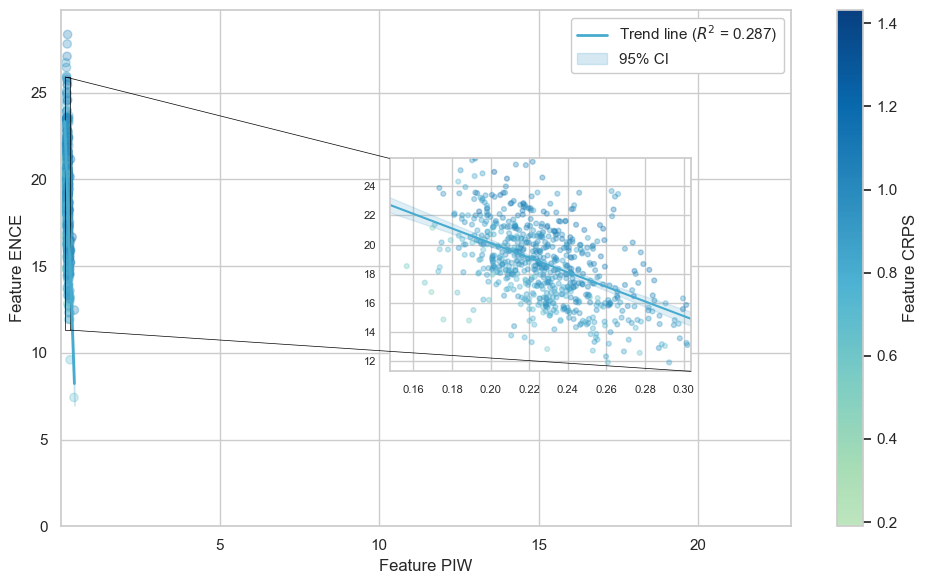
\includegraphics[width=\linewidth]{images/MCD/mcd_methylation/methyl_scatter_piw_ence_zoom_OOD.png}
        \caption{Out-of-Sample data.}
        \label{fig:mcd_methylation_piw_ence_out}
    \end{subfigure}
    \caption[MCD Methylation PIW-ENCE scatter plots]{Methylation feature-wise scatter plots between PIW and ENCE with CRPS as colour gradient, calculated from Monte Carlo Dropout samples.}
    \label{fig:mcd_methylation_piw_ence}
\end{figure}

This behaviour differs from Drug Response, Proteomics and Transcriptomics, where the in-sample relationship between sharpness and calibration follows the opposite direction and sharper features tend to be more miscalibrated. Methylation is closer to Metabolomics and CRISPR-Cas9 in-sample, but with a more extreme spread of PIW values alongside ENCE. This is shown in Figure \ref{fig:mcd_methylation_piw_ence}(a), where PIW generally increases with ENCE, with an \(R^2\) of 0.679. Larger CRPS values are mostly restricted to features for which both PIW and ENCE are high. However, the same panel also shows a group of low-PIW features following the opposite tendency, indicating that some sharper in-sample features are also poorly calibrated.

Out-of-sample, Methylation has a much lower feature-wise mean PIW. As previously mentioned, many of its feature-level predictions have predictive variance close to zero. Figure \ref{fig:mcd_methylation_piw_ence}(b) reflects this shift, showing very small PIW values. Unlike in-sample, PIW no longer explains ENCE, with an \(R^2\) of 0.016, as the retained features have ENCE values between 4.91 and 34.7 regardless of their PIW. Out-of-sample Methylation is therefore overconfident across its features, not only for the sharpest ones.

\begin{figure}[!ht]
    \centering
    \begin{subfigure}{0.48\linewidth}
        \centering
        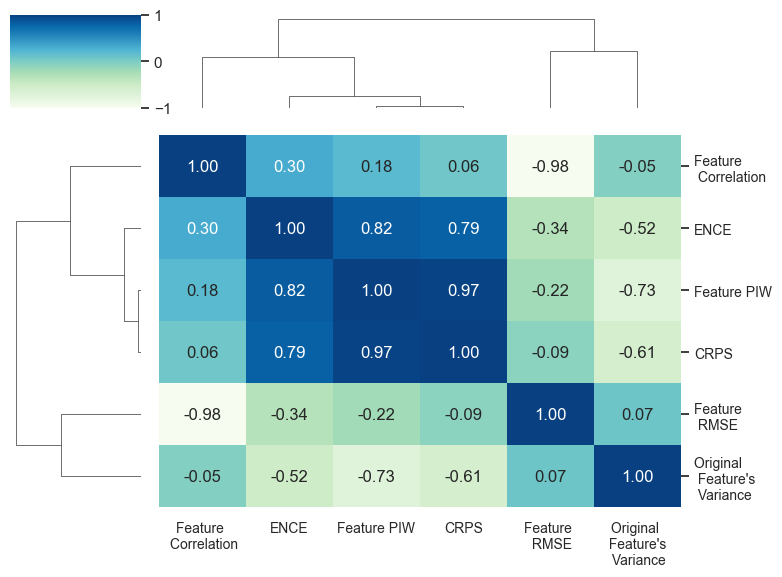
\includegraphics[width=\linewidth]{images/MCD/mcd_methylation/mcd_methylation_cluster_map.png}
        \caption{In-Sample data.}
        \label{fig:mcd_methylation_cluster_map_in}
    \end{subfigure}
    \hfill
    \begin{subfigure}{0.48\linewidth}
        \centering
        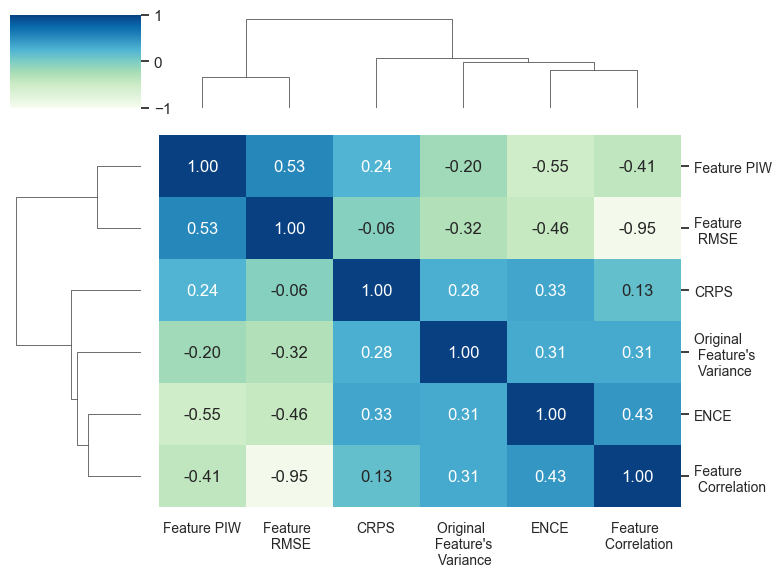
\includegraphics[width=\linewidth]{images/MCD/mcd_methylation/mcd_methylation_cluster_map_OOD.png}
        \caption{Out-of-Sample data.}
        \label{fig:mcd_methylation_cluster_map_out}
    \end{subfigure}
    \caption[MCD Methylation uncertainty correlation cluster-map]{Methylation Pearson correlation cluster-map between feature-wise Monte Carlo Dropout uncertainty metrics, reconstruction-error metrics, missing-value percentage and original feature variance.}
    \label{fig:mcd_methylation_cluster_map}
\end{figure}


The relationship between uncertainty and reconstruction error also changes between the two settings. In-sample, PIW is weakly and ENCE moderately negatively associated with RMSE, with correlations of -0.21 and -0.34, respectively. PIW also shows a strong negative correlation with the original feature variance, at -0.73, while ENCE and CRPS show moderate negative correlations, at -0.52 and -0.60. Features with higher variance tend to have narrower predictive intervals, lower calibration error and lower scoring-rule values in-sample.

Out-of-sample, PIW becomes moderately positively associated with RMSE, with a correlation of 0.38, while ENCE becomes moderately positively associated with RMSE, at 0.68, so the features that are reconstructed worst are also the most miscalibrated. The association with the original feature variance weakens to -0.27 for PIW and disappears for ENCE and CRPS, at -0.01 and 0.04. 

Methylation therefore follows the pattern observed across the continuous omics, where uncertainty does not increase enough for the features with poorer reconstruction. Out-of-sample, PIW increases only moderately with RMSE, while ENCE increases more strongly with it.


The calibration curves in Figure \ref{fig:mcd_methylation_calibration_curves}(a) exemplify well calibrated features. For the six features displayed, most RMV bins closely match the corresponding mean RMSE values. Despite this, and as mentioned previously, Methylation still contains features with large ENCE values, as shown in Figure \ref{fig:mcd_methylation_calibration_curves}(b). Even these features have a clearly lower discrepancy between RMV and RMSE than those displayed in Figure \ref{fig:metabolomics_calibration_curves}. These plots generalise to the ENCE values of the remaining continuous omics, where features with ENCE or ECE closer to 0 follow curves similar to those in Figure \ref{fig:mcd_methylation_calibration_curves}(a).

\begin{figure}[!ht]
    \centering
    \begin{subfigure}{0.48\linewidth}
        \centering
        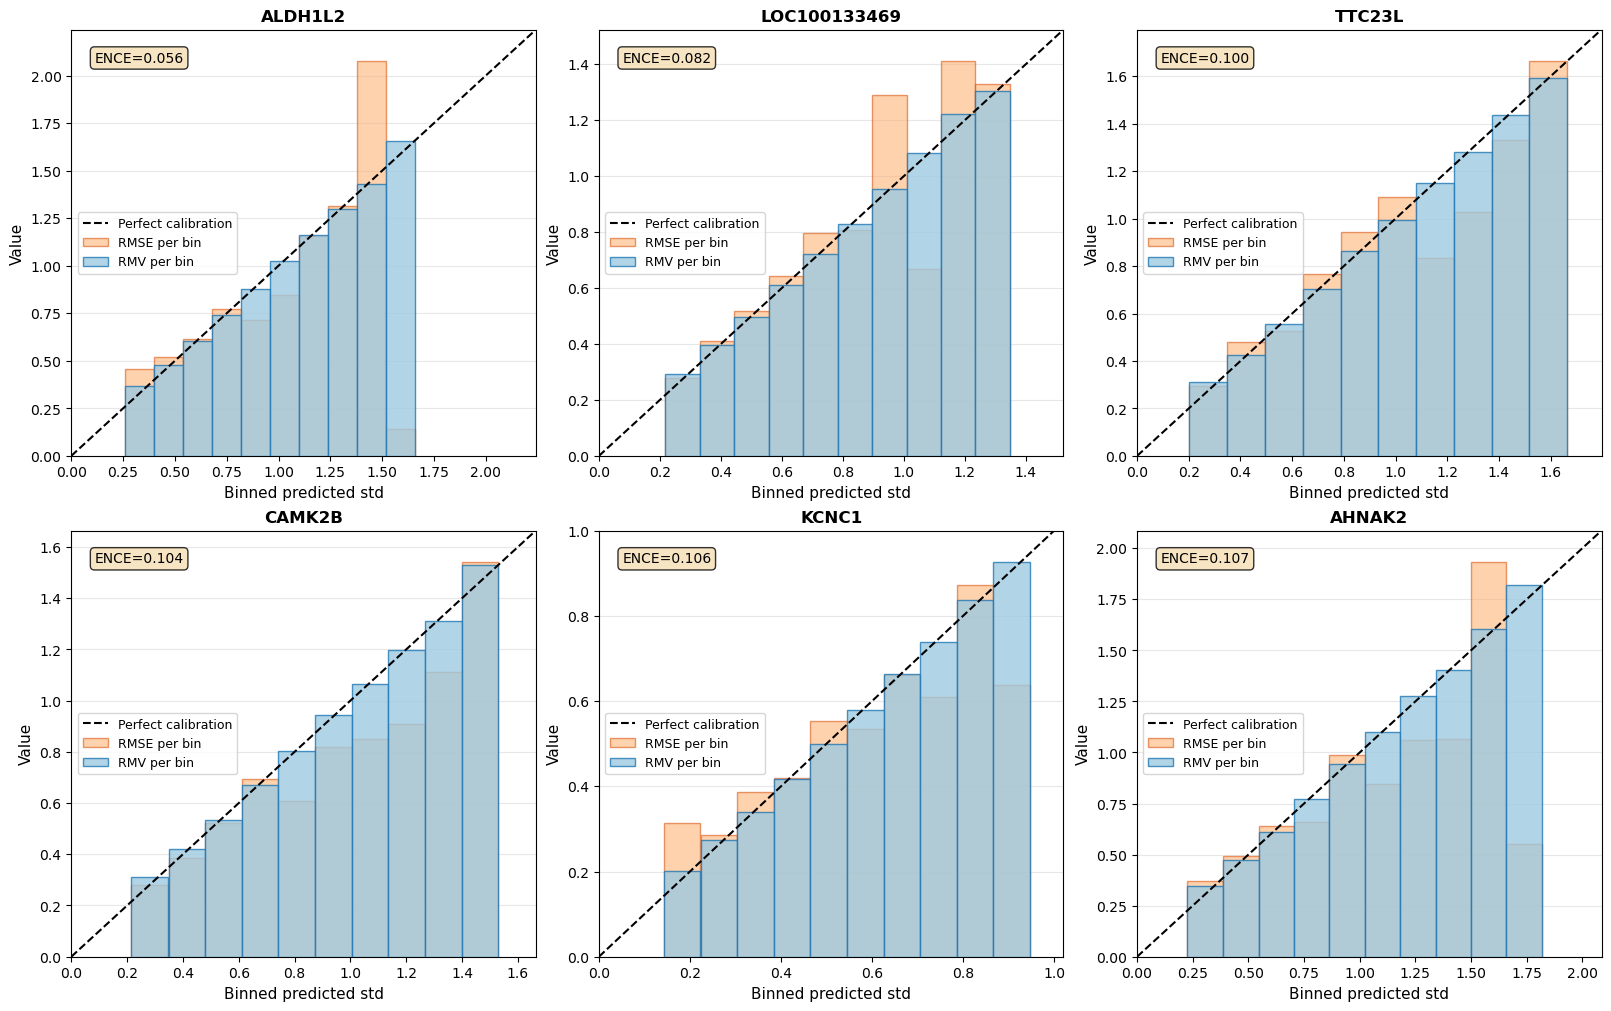
\includegraphics[width=\linewidth]{images/MCD/mcd_methylation/methylation_calibration_curves_smallest_ece_MCD.png}
        \caption{Smallest calibration errors.}
        \label{fig:mcd_methylation_calibration_curves_smallest}
    \end{subfigure}
    \hfill
    \begin{subfigure}{0.48\linewidth}
        \centering
        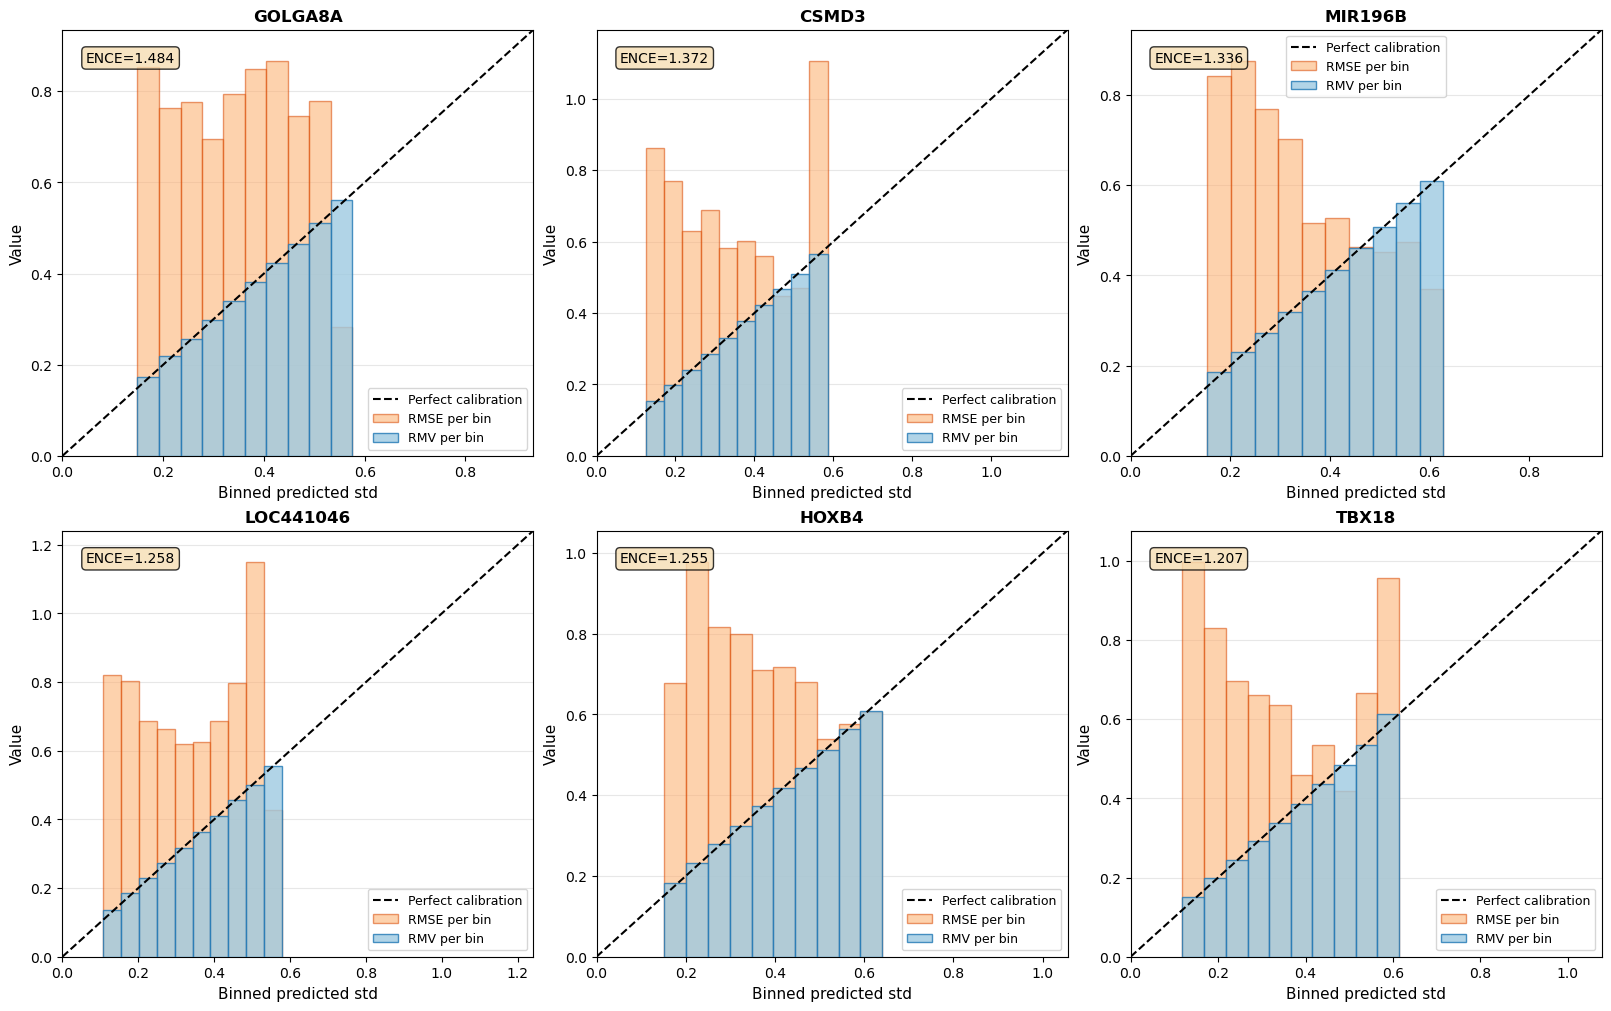
\includegraphics[width=\linewidth]{images/MCD/mcd_methylation/methylation_calibration_curves_largest_ece_MCD.png}
        \caption{Largest calibration errors.}
        \label{fig:mcd_methylation_calibration_curves_largest}
    \end{subfigure}
    \caption[MCD Methylation calibration curves]{Methylation calibration curves for the features with the smallest and largest calibration errors under Monte Carlo Dropout.}
    \label{fig:mcd_methylation_calibration_curves}
\end{figure}

\subsubsection{Proteomics}

Proteomics contrasts with Methylation in that it better aligns with the remaining continuous omics while also allowing the analysis of the relationship between the feature-wise percentage of missing values and the uncertainty metrics considered. While Methylation represents an extreme shift between in-sample and out-of-sample behaviour, Proteomics is closer to the general continuous-omic pattern, especially in the out-of-sample reconstructions.

\begin{figure}[!ht]
    \centering
    \begin{subfigure}{0.48\linewidth}
        \centering
        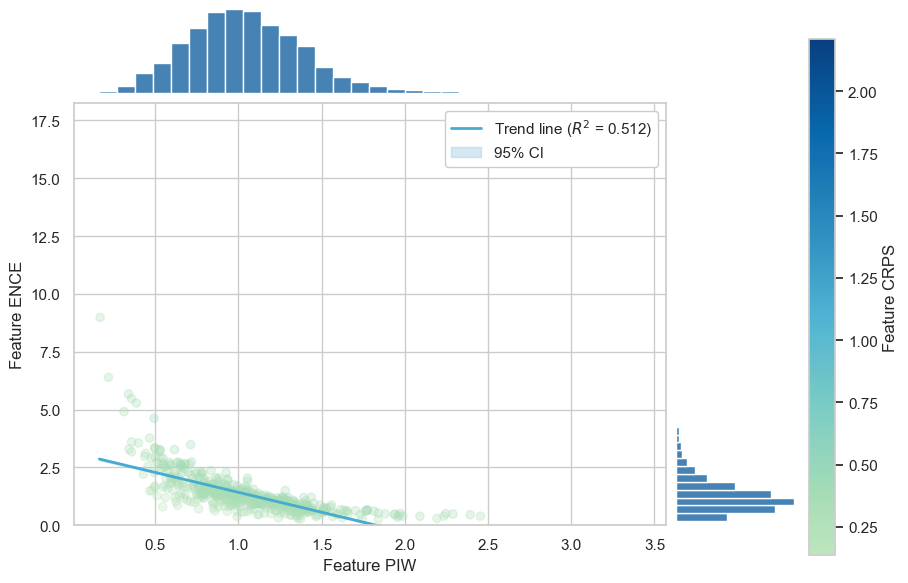
\includegraphics[width=\linewidth]{images/MCD/mcd_proteomics/prot_scatter_piw_ence.png}
        \caption{In-Sample data.}
        \label{fig:mcd_proteomics_piw_ence_in}
    \end{subfigure}
    \hfill
    \begin{subfigure}{0.48\linewidth}
        \centering
        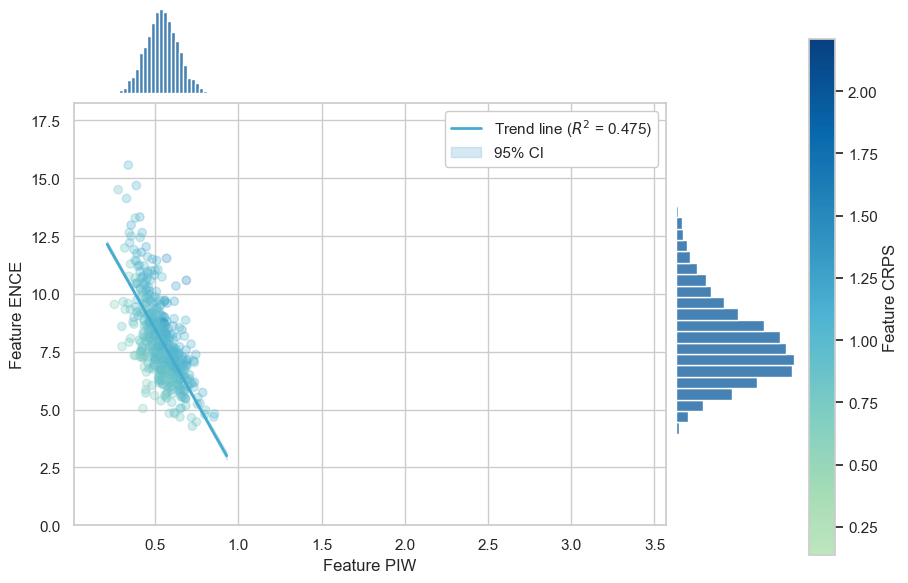
\includegraphics[width=\linewidth]{images/MCD/mcd_proteomics/prot_scatter_piw_ence_OOD.png}
        \caption{Out-of-Sample data.}
        \label{fig:mcd_proteomics_piw_ence_out}
    \end{subfigure}
    \caption[MCD Proteomics PIW-ENCE scatter plots]{Proteomics feature-wise scatter plots between PIW and ENCE with CRPS as colour gradient, calculated from Monte Carlo Dropout samples.}
    \label{fig:mcd_proteomics_piw_ence}
\end{figure}

As shown in Figure \ref{fig:mcd_proteomics_piw_ence}(a), Proteomics has a narrower in-sample sharpness profile than Methylation. Its PIW values are lower than those observed for Methylation and CRISPR-Cas9, and its feature-wise sharpness distribution is closer to Drug Response. Overall, this lower predictive variability is accompanied by relatively good calibration for most features. However, in-sample Proteomics still follows a similar pattern to Drug Response and Transcriptomics among the features with worse calibration, where sharper features tend to be more miscalibrated. Here, features with lower PIW are overconfident in their predictions relative to their prediction error, leading to higher ENCE values.

\begin{figure}[!ht]
    \centering
    \begin{subfigure}{0.48\linewidth}
        \centering
        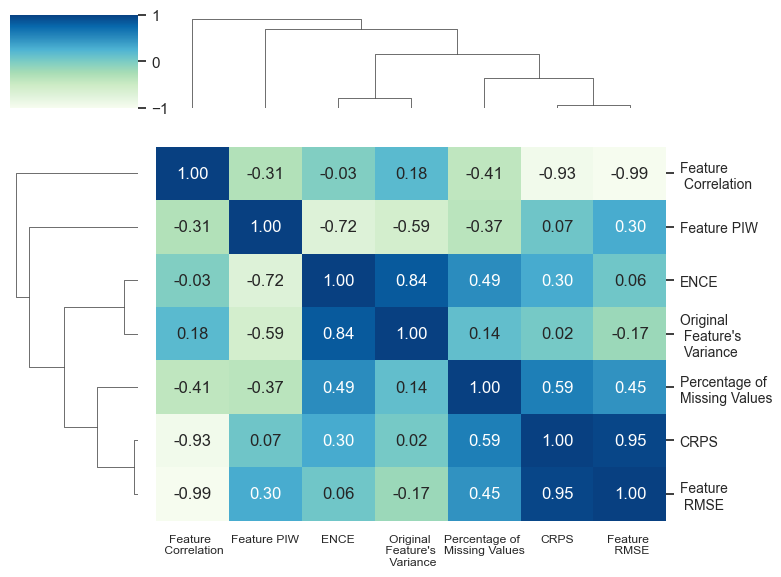
\includegraphics[width=\linewidth]{images/MCD/mcd_proteomics/mcd_proteomics_cluster_map.png}
        \caption{In-Sample data.}
        \label{fig:mcd_proteomics_corr_in}
    \end{subfigure}
    \hfill
    \begin{subfigure}{0.48\linewidth}
        \centering
        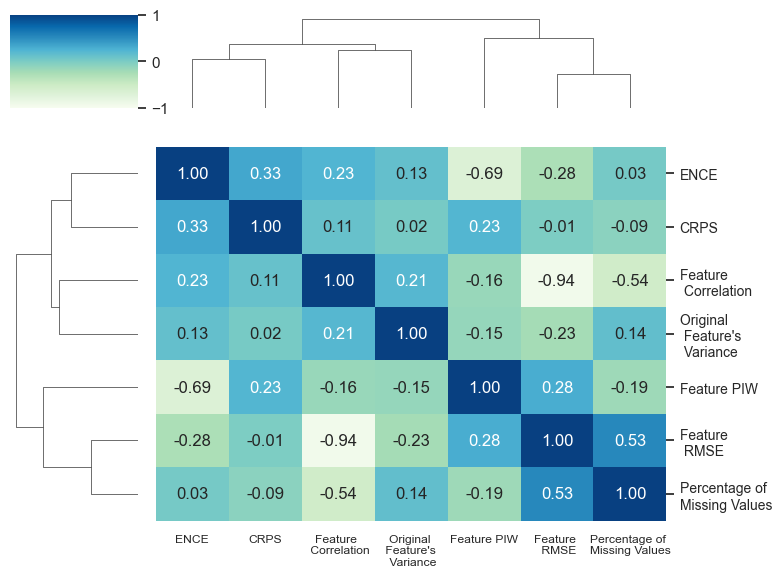
\includegraphics[width=\linewidth]{images/MCD/mcd_proteomics/mcd_proteomics_cluster_map_OOD.png}
        \caption{Out-of-Sample data.}
        \label{fig:mcd_proteomics_corr_out}
    \end{subfigure}
    \caption[MCD Proteomics uncertainty correlation cluster-map]{Proteomics Pearson correlation cluster-map between feature-wise Monte Carlo Dropout uncertainty metrics, reconstruction-error metrics, missing-value percentage and original feature variance.}
    \label{fig:mcd_proteomics_corr}
\end{figure}

As seen in Figure \ref{fig:mcd_proteomics_corr}(a), in-sample PIW has a weak positive correlation with RMSE, at 0.30, while ENCE has a very weak positive correlation with RMSE, at 0.06.

When compared to other omics such as Metabolomics or Drug Response, missingness is more clearly associated with the remaining uncertainty metrics. In-sample feature-wise missing-value percentage has a moderate positive correlation with ENCE and CRPS, with correlations of 0.49 and 0.59, respectively, and a moderate negative correlation with PIW, at -0.37. This suggests that features with more missing values tend to have poorer calibration and scoring, while also having smaller PIW. Similarly, the feature variance of the original dataset exhibits a strong positive correlation with ENCE, at 0.84, and a moderate negative correlation with PIW, at -0.59. Features with larger variance tend to have narrower predictive distributions while also showing larger calibration error. The model therefore appears more overconfident for high-variance proteomics features, where the larger data variability is not reflected in the estimated epistemic uncertainty.

Out-of-sample, Proteomics retains a similar structure to the one observed in-sample. As seen in Figures \ref{fig:mcd_proteomics_piw_ence}(b) and \ref{fig:mcd_proteomics_corr}(b), PIW and ENCE remain moderately negatively correlated, at -0.49, while PIW becomes almost unrelated to RMSE, at 0.10. Missingness keeps a similar association with calibration and scoring, with correlations of 0.50 with ENCE and 0.45 with CRPS, and CRPS remains strongly associated with RMSE, at 0.94. The main change concerns ENCE. Its association with RMSE, almost absent in-sample at 0.06, becomes moderately positive out-of-sample at 0.69, while its strong in-sample association with the original feature variance disappears, at -0.05. Out-of-sample, calibration error is therefore driven by reconstruction error rather than by feature variance. Overall, the persistence of the negative PIW-ENCE relationship points to overconfidence, as the features with the narrowest predictive distributions are often those for which the predicted uncertainty has the greatest mismatch with the observed reconstruction behaviour.



\section{Discussion and Comparison of the Uncertainty Estimation Methods}

%Faz sentido colocar um plot (bar chart?) que mostre os valores de sharpness, calibration, scoring entre os dois métodos?
%Devo ser mais in depth na comparação?

The two uncertainty estimation strategies used provide complementary views of MOSA's reconstruction uncertainty. Note that the comparison between these two different methods should not be interpreted as a comparison between two equal estimators of the same uncertainty. Additionally, these methods should be viewed as estimates of different sources of predictive uncertainty and not as direct decompositions of the model's true uncertainty.


In-sample, Monte Carlo Dropout produces much wider predictive intervals than Latent Space Sampling for every continuous omic, most markedly for Methylation, Metabolomics and CRISPR-Cas9. In comparison, Latent Space Sampling produces both narrower and more homogeneous predictive distributions. Out-of-sample the difference shrinks, and it is reversed for Methylation and Transcriptomics, where the Latent Space Sampling intervals are wider. The in-sample pattern suggests that aleatoric uncertainty has a considerably smaller impact on the model's reconstruction than epistemic uncertainty. 

Despite the different magnitudes of sharpness values, both methods display a mismatch between predictive uncertainty and reconstruction error. For Latent Space Sampling, the narrow predictive intervals are accompanied by high ENCE values across all continuous omics. The prevalence of these two characteristics is particularly important as narrow predictive intervals are only desirable when accompanied by accurate reconstructions. Here, the calibration values suggest that this precision of the decoded latent-space samples corresponds to overconfident reconstructions. Monte Carlo Dropout provides a different picture in some in-sample datasets, as this method's samples overall provide wider predictive intervals accompanied by lower calibration values. Despite this, there are still multiple continuous features with ENCE larger than one. In several out-of-sample reconstructions, the predictive intervals become narrower, while calibration and scoring-rule values tend to deteriorate. Out-of-sample, the two methods nevertheless reach similar scoring-rule values, with mean CRPS values between 0.54 and 0.77 that differ by less than 0.03 between methods for every continuous omic. The epistemic uncertainty estimated through dropout does not consistently increase in the cases where reconstruction is more difficult, which would be expected as prediction error does increase for out-of-sample data reconstructions.

Copy number contrasts with the continuous omics for both estimation methods. Latent Space Sampling estimations have entropy close to zero both in-sample and out-of-sample. However, unlike the continuous datasets, these features are not uniformly miscalibrated. This difference is likely influenced by the low diversity of the original Copy number data, where many features are dominated by one or two classes. Contrasting with the continuous datasets, features with lower entropy tend to have lower ECE values. Monte Carlo Dropout estimates have a higher entropy for Copy number than Latent Space Sampling, with means of 0.265 against 0.0242 in-sample and 0.158 against 0.0343 out-of-sample, but lower calibration errors and scoring-rule values in both settings, with mean ECE of 0.0767 against 0.246 in-sample and 0.264 against 0.351 out-of-sample, and mean Log Score of 1.31 against 7.52 and 5.15 against 10.6. 

Comparison between the in-sample and out-of-sample metrics is also relevant to assess the possible impact of overfitting, although this cannot by itself prove the presence of overfitting. Overfit machine learning models learn patterns in the training data but struggle to generalise those patterns to new observations. The gap observed between in-sample and out-of-sample data reconstructions is therefore a useful proxy for this possibility. In particular, cases where out-of-sample data shows poor reconstruction without an increase in sharpness or an improvement in calibration values are consistent with an overconfident model that does not correctly express the true predicted uncertainty when reconstructing outside of training data. Similarly, when looking at each omic dataset individually, some relationships between the uncertainty metrics and RMSE, missingness and feature variance change between in-sample and out-of-sample data, while others persist. Missingness remains associated with calibration in Proteomics under both methods, and out-of-sample the most poorly reconstructed features tend to be the most miscalibrated. The correlation between ENCE and RMSE ranges from 0.57 to 0.78 under Latent Space Sampling for all continuous omics except CRISPR-Cas9, at 0.19, and from 0.54 to 0.74 under Monte Carlo Dropout. This suggests that the uncertainty estimates are partially tied to properties of the training reconstruction, as they do not generalise uniformly for the held-out values.

These patterns should be interpreted with caution as deterioration from in-sample to out-of-sample reconstructions can arise from several sources besides overfitting. This includes weaker cross-omic signal for particular datasets, high feature noise, the structure of missing values per dataset or limited sample size in the held-out subset. While the uncertainty analysis done provides potential evidence of overfitting behaviour, it is not a direct diagnosis of overfitting. A stronger conclusion would require additional tests; these include explicit comparison of training and validation losses across epochs, cross-validation across multiple folds, regularisation sensitivity analysis or evaluation on independent external datasets.